\documentclass[twoside]{book}

% Packages required by doxygen
\usepackage{fixltx2e}
\usepackage{calc}
\usepackage{doxygen}
\usepackage[export]{adjustbox} % also loads graphicx
\usepackage{graphicx}
\usepackage[utf8]{inputenc}
\usepackage{makeidx}
\usepackage{multicol}
\usepackage{multirow}
\PassOptionsToPackage{warn}{textcomp}
\usepackage{textcomp}
\usepackage[nointegrals]{wasysym}
\usepackage[table]{xcolor}

% Font selection
\usepackage[T1]{fontenc}
\usepackage[scaled=.90]{helvet}
\usepackage{courier}
\usepackage{amssymb}
\usepackage{sectsty}
\renewcommand{\familydefault}{\sfdefault}
\allsectionsfont{%
  \fontseries{bc}\selectfont%
  \color{darkgray}%
}
\renewcommand{\DoxyLabelFont}{%
  \fontseries{bc}\selectfont%
  \color{darkgray}%
}
\newcommand{\+}{\discretionary{\mbox{\scriptsize$\hookleftarrow$}}{}{}}

% Page & text layout
\usepackage{geometry}
\geometry{%
  a4paper,%
  top=2.5cm,%
  bottom=2.5cm,%
  left=2.5cm,%
  right=2.5cm%
}
\tolerance=750
\hfuzz=15pt
\hbadness=750
\setlength{\emergencystretch}{15pt}
\setlength{\parindent}{0cm}
\setlength{\parskip}{3ex plus 2ex minus 2ex}
\makeatletter
\renewcommand{\paragraph}{%
  \@startsection{paragraph}{4}{0ex}{-1.0ex}{1.0ex}{%
    \normalfont\normalsize\bfseries\SS@parafont%
  }%
}
\renewcommand{\subparagraph}{%
  \@startsection{subparagraph}{5}{0ex}{-1.0ex}{1.0ex}{%
    \normalfont\normalsize\bfseries\SS@subparafont%
  }%
}
\makeatother

% Headers & footers
\usepackage{fancyhdr}
\pagestyle{fancyplain}
\fancyhead[LE]{\fancyplain{}{\bfseries\thepage}}
\fancyhead[CE]{\fancyplain{}{}}
\fancyhead[RE]{\fancyplain{}{\bfseries\leftmark}}
\fancyhead[LO]{\fancyplain{}{\bfseries\rightmark}}
\fancyhead[CO]{\fancyplain{}{}}
\fancyhead[RO]{\fancyplain{}{\bfseries\thepage}}
\fancyfoot[LE]{\fancyplain{}{}}
\fancyfoot[CE]{\fancyplain{}{}}
\fancyfoot[RE]{\fancyplain{}{\bfseries\scriptsize Generated by Doxygen }}
\fancyfoot[LO]{\fancyplain{}{\bfseries\scriptsize Generated by Doxygen }}
\fancyfoot[CO]{\fancyplain{}{}}
\fancyfoot[RO]{\fancyplain{}{}}
\renewcommand{\footrulewidth}{0.4pt}
\renewcommand{\chaptermark}[1]{%
  \markboth{#1}{}%
}
\renewcommand{\sectionmark}[1]{%
  \markright{\thesection\ #1}%
}

% Indices & bibliography
\usepackage{natbib}
\usepackage[titles]{tocloft}
\setcounter{tocdepth}{3}
\setcounter{secnumdepth}{5}
\makeindex

% Hyperlinks (required, but should be loaded last)
\usepackage{ifpdf}
\ifpdf
  \usepackage[pdftex,pagebackref=true]{hyperref}
\else
  \usepackage[ps2pdf,pagebackref=true]{hyperref}
\fi
\hypersetup{%
  colorlinks=true,%
  linkcolor=blue,%
  citecolor=blue,%
  unicode%
}

% Custom commands
\newcommand{\clearemptydoublepage}{%
  \newpage{\pagestyle{empty}\cleardoublepage}%
}

\usepackage{caption}
\captionsetup{labelsep=space,justification=centering,font={bf},singlelinecheck=off,skip=4pt,position=top}

%===== C O N T E N T S =====

\begin{document}

% Titlepage & ToC
\hypersetup{pageanchor=false,
             bookmarksnumbered=true,
             pdfencoding=unicode
            }
\pagenumbering{alph}
\begin{titlepage}
\vspace*{7cm}
\begin{center}%
{\Large My Project }\\
\vspace*{1cm}
{\large Generated by Doxygen 1.8.13}\\
\end{center}
\end{titlepage}
\clearemptydoublepage
\pagenumbering{roman}
\tableofcontents
\clearemptydoublepage
\pagenumbering{arabic}
\hypersetup{pageanchor=true}

%--- Begin generated contents ---
\chapter{Data Structure Index}
\section{Data Structures}
Here are the data structures with brief descriptions\+:\begin{DoxyCompactList}
\item\contentsline{section}{\hyperlink{struct_v_g_a__t}{V\+G\+A\+\_\+t} }{\pageref{struct_v_g_a__t}}{}
\end{DoxyCompactList}

\chapter{File Index}
\section{File List}
Here is a list of all documented files with brief descriptions\+:\begin{DoxyCompactList}
\item\contentsline{section}{A\+P\+I/{\bfseries A\+P\+I\+\_\+\+Draw.\+c} }{\pageref{_a_p_i___draw_8c}}{}
\item\contentsline{section}{A\+P\+I/\hyperlink{_a_p_i___draw_8h}{A\+P\+I\+\_\+\+Draw.\+h} \\*Common definition used by all files and public A\+PI }{\pageref{_a_p_i___draw_8h}}{}
\item\contentsline{section}{A\+P\+I/{\bfseries A\+P\+I\+\_\+\+I\+O.\+c} }{\pageref{_a_p_i___i_o_8c}}{}
\item\contentsline{section}{A\+P\+I/\hyperlink{_a_p_i___i_o_8h}{A\+P\+I\+\_\+\+I\+O.\+h} \\*Common definition used by all files and public A\+PI }{\pageref{_a_p_i___i_o_8h}}{}
\end{DoxyCompactList}

\chapter{Data Structure Documentation}
\hypertarget{struct_b_i_t_m_a_p}{}\section{B\+I\+T\+M\+AP Struct Reference}
\label{struct_b_i_t_m_a_p}\index{B\+I\+T\+M\+AP@{B\+I\+T\+M\+AP}}
\subsection*{Data Fields}
\begin{DoxyCompactItemize}
\item 
\mbox{\Hypertarget{struct_b_i_t_m_a_p_a4dde988b1b2adba65ae3efa69f65d960}\label{struct_b_i_t_m_a_p_a4dde988b1b2adba65ae3efa69f65d960}} 
uint16\+\_\+t {\bfseries x}
\item 
\mbox{\Hypertarget{struct_b_i_t_m_a_p_ab0580f504a7428539be299fa71565f30}\label{struct_b_i_t_m_a_p_ab0580f504a7428539be299fa71565f30}} 
uint16\+\_\+t {\bfseries y}
\item 
\mbox{\Hypertarget{struct_b_i_t_m_a_p_a02b2be7b8ce086893453d390c5fdcf1d}\label{struct_b_i_t_m_a_p_a02b2be7b8ce086893453d390c5fdcf1d}} 
uint16\+\_\+t {\bfseries bitmap}
\end{DoxyCompactItemize}


\subsection{Detailed Description}


Definition at line 79 of file A\+P\+I\+\_\+\+Draw.\+h.



The documentation for this struct was generated from the following file\+:\begin{DoxyCompactItemize}
\item 
A\+P\+I/\hyperlink{_a_p_i___draw_8h}{A\+P\+I\+\_\+\+Draw.\+h}\end{DoxyCompactItemize}

\hypertarget{struct_c_o_m_m_a_n_d__t}{}\section{C\+O\+M\+M\+A\+N\+D\+\_\+t Struct Reference}
\label{struct_c_o_m_m_a_n_d__t}\index{C\+O\+M\+M\+A\+N\+D\+\_\+t@{C\+O\+M\+M\+A\+N\+D\+\_\+t}}


Structure for the buffers.  




{\ttfamily \#include $<$A\+P\+I\+\_\+\+I\+O.\+h$>$}

\subsection*{Data Fields}
\begin{DoxyCompactItemize}
\item 
\mbox{\Hypertarget{struct_c_o_m_m_a_n_d__t_a3ca56d05670fa13929584cd8aebae252}\label{struct_c_o_m_m_a_n_d__t_a3ca56d05670fa13929584cd8aebae252}} 
char \hyperlink{struct_c_o_m_m_a_n_d__t_a3ca56d05670fa13929584cd8aebae252}{buff} \mbox{[}\hyperlink{_a_p_i___i_o_8h_a9e8aaf9c28f704136d8fc1ba043b6bf5}{S\+T\+R\+\_\+\+L\+E\+N\+G\+TH}\mbox{]}
\begin{DoxyCompactList}\small\item\em fill buffer \end{DoxyCompactList}\item 
\mbox{\Hypertarget{struct_c_o_m_m_a_n_d__t_a106c2825d202a4530656fcd385d0c04b}\label{struct_c_o_m_m_a_n_d__t_a106c2825d202a4530656fcd385d0c04b}} 
char \hyperlink{struct_c_o_m_m_a_n_d__t_a106c2825d202a4530656fcd385d0c04b}{type} \mbox{[}\hyperlink{_a_p_i___i_o_8h_a7be6924e0d85f3f82149ea31cca36887}{T\+Y\+P\+E\+\_\+\+L\+E\+N\+G\+TH}\mbox{]}
\begin{DoxyCompactList}\small\item\em type of the \end{DoxyCompactList}\item 
\mbox{\Hypertarget{struct_c_o_m_m_a_n_d__t_adc64ccb7538429fe78e3fe0139267370}\label{struct_c_o_m_m_a_n_d__t_adc64ccb7538429fe78e3fe0139267370}} 
uint8\+\_\+t {\bfseries error}
\end{DoxyCompactItemize}


\subsection{Detailed Description}
Structure for the buffers. 

Definition at line 266 of file A\+P\+I\+\_\+\+I\+O.\+h.



The documentation for this struct was generated from the following file\+:\begin{DoxyCompactItemize}
\item 
A\+P\+I/\hyperlink{_a_p_i___i_o_8h}{A\+P\+I\+\_\+\+I\+O.\+h}\end{DoxyCompactItemize}

\hypertarget{struct_e_l_l_i_p_s_e}{}\section{E\+L\+L\+I\+P\+SE Struct Reference}
\label{struct_e_l_l_i_p_s_e}\index{E\+L\+L\+I\+P\+SE@{E\+L\+L\+I\+P\+SE}}
\subsection*{Data Fields}
\begin{DoxyCompactItemize}
\item 
\mbox{\Hypertarget{struct_e_l_l_i_p_s_e_a949409b5dddb52782ff2cb935f4640fa}\label{struct_e_l_l_i_p_s_e_a949409b5dddb52782ff2cb935f4640fa}} 
uint16\+\_\+t \hyperlink{struct_e_l_l_i_p_s_e_a949409b5dddb52782ff2cb935f4640fa}{xp}
\begin{DoxyCompactList}\small\item\em horizontal begin position of the line \end{DoxyCompactList}\item 
\mbox{\Hypertarget{struct_e_l_l_i_p_s_e_a59b81f7ac350cf9080d3d0b767580e4d}\label{struct_e_l_l_i_p_s_e_a59b81f7ac350cf9080d3d0b767580e4d}} 
uint16\+\_\+t \hyperlink{struct_e_l_l_i_p_s_e_a59b81f7ac350cf9080d3d0b767580e4d}{yp}
\begin{DoxyCompactList}\small\item\em horizontal begin position of the line \end{DoxyCompactList}\item 
\mbox{\Hypertarget{struct_e_l_l_i_p_s_e_ad0eab1042455a2067c812ab8071d5376}\label{struct_e_l_l_i_p_s_e_ad0eab1042455a2067c812ab8071d5376}} 
uint16\+\_\+t \hyperlink{struct_e_l_l_i_p_s_e_ad0eab1042455a2067c812ab8071d5376}{width}
\begin{DoxyCompactList}\small\item\em horizontal begin position of the line \end{DoxyCompactList}\item 
\mbox{\Hypertarget{struct_e_l_l_i_p_s_e_a81c9f8d0b8c3b49d770be14dbe9f0d37}\label{struct_e_l_l_i_p_s_e_a81c9f8d0b8c3b49d770be14dbe9f0d37}} 
uint16\+\_\+t \hyperlink{struct_e_l_l_i_p_s_e_a81c9f8d0b8c3b49d770be14dbe9f0d37}{height}
\begin{DoxyCompactList}\small\item\em horizontal begin position of the line \end{DoxyCompactList}\item 
\mbox{\Hypertarget{struct_e_l_l_i_p_s_e_a2ffb43952012965173826ee9554c864a}\label{struct_e_l_l_i_p_s_e_a2ffb43952012965173826ee9554c864a}} 
uint8\+\_\+t \hyperlink{struct_e_l_l_i_p_s_e_a2ffb43952012965173826ee9554c864a}{fill}
\begin{DoxyCompactList}\small\item\em horizontal begin position of the line \end{DoxyCompactList}\item 
\mbox{\Hypertarget{struct_e_l_l_i_p_s_e_a21caa4b27a71b7967f1a2d64f196a674}\label{struct_e_l_l_i_p_s_e_a21caa4b27a71b7967f1a2d64f196a674}} 
uint8\+\_\+t \hyperlink{struct_e_l_l_i_p_s_e_a21caa4b27a71b7967f1a2d64f196a674}{colint}
\begin{DoxyCompactList}\small\item\em horizontal begin position of the line \end{DoxyCompactList}\end{DoxyCompactItemize}


\subsection{Detailed Description}


Definition at line 47 of file A\+P\+I\+\_\+\+Draw.\+h.



The documentation for this struct was generated from the following file\+:\begin{DoxyCompactItemize}
\item 
A\+P\+I/\hyperlink{_a_p_i___draw_8h}{A\+P\+I\+\_\+\+Draw.\+h}\end{DoxyCompactItemize}

\hypertarget{struct_l_i_n_e}{}\section{L\+I\+NE Struct Reference}
\label{struct_l_i_n_e}\index{L\+I\+NE@{L\+I\+NE}}


Structure for line parameters.  




{\ttfamily \#include $<$A\+P\+I\+\_\+\+Draw.\+h$>$}

\subsection*{Data Fields}
\begin{DoxyCompactItemize}
\item 
\mbox{\Hypertarget{struct_l_i_n_e_aedb5fdfe3c1d1a915b668ba7f3950753}\label{struct_l_i_n_e_aedb5fdfe3c1d1a915b668ba7f3950753}} 
uint16\+\_\+t \hyperlink{struct_l_i_n_e_aedb5fdfe3c1d1a915b668ba7f3950753}{x1}
\begin{DoxyCompactList}\small\item\em horizontal begin position of the line \end{DoxyCompactList}\item 
\mbox{\Hypertarget{struct_l_i_n_e_a47ada631c22a9d40348069145654f255}\label{struct_l_i_n_e_a47ada631c22a9d40348069145654f255}} 
uint16\+\_\+t \hyperlink{struct_l_i_n_e_a47ada631c22a9d40348069145654f255}{y1}
\begin{DoxyCompactList}\small\item\em vertical begin position of the line \end{DoxyCompactList}\item 
\mbox{\Hypertarget{struct_l_i_n_e_ac5bc000f8954f38b7a641a485a26bae7}\label{struct_l_i_n_e_ac5bc000f8954f38b7a641a485a26bae7}} 
uint16\+\_\+t \hyperlink{struct_l_i_n_e_ac5bc000f8954f38b7a641a485a26bae7}{x2}
\begin{DoxyCompactList}\small\item\em horizontal end position of the line \end{DoxyCompactList}\item 
\mbox{\Hypertarget{struct_l_i_n_e_aa377184ba406b3f0c4ac18c935378204}\label{struct_l_i_n_e_aa377184ba406b3f0c4ac18c935378204}} 
uint16\+\_\+t \hyperlink{struct_l_i_n_e_aa377184ba406b3f0c4ac18c935378204}{y2}
\begin{DoxyCompactList}\small\item\em vertical end position of the line \end{DoxyCompactList}\item 
\mbox{\Hypertarget{struct_l_i_n_e_a09a2a45f731b02946ff6d3cd15c1a476}\label{struct_l_i_n_e_a09a2a45f731b02946ff6d3cd15c1a476}} 
uint8\+\_\+t \hyperlink{struct_l_i_n_e_a09a2a45f731b02946ff6d3cd15c1a476}{width}
\begin{DoxyCompactList}\small\item\em weight of the line \end{DoxyCompactList}\item 
\mbox{\Hypertarget{struct_l_i_n_e_a21caa4b27a71b7967f1a2d64f196a674}\label{struct_l_i_n_e_a21caa4b27a71b7967f1a2d64f196a674}} 
uint8\+\_\+t \hyperlink{struct_l_i_n_e_a21caa4b27a71b7967f1a2d64f196a674}{colint}
\begin{DoxyCompactList}\small\item\em color of the line \end{DoxyCompactList}\end{DoxyCompactItemize}


\subsection{Detailed Description}
Structure for line parameters. 

Definition at line 24 of file A\+P\+I\+\_\+\+Draw.\+h.



The documentation for this struct was generated from the following file\+:\begin{DoxyCompactItemize}
\item 
A\+P\+I/\hyperlink{_a_p_i___draw_8h}{A\+P\+I\+\_\+\+Draw.\+h}\end{DoxyCompactItemize}

\hypertarget{struct_s_q_u_a_r_e}{}\section{S\+Q\+U\+A\+RE Struct Reference}
\label{struct_s_q_u_a_r_e}\index{S\+Q\+U\+A\+RE@{S\+Q\+U\+A\+RE}}


Structure for rectangle parameters.  




{\ttfamily \#include $<$A\+P\+I\+\_\+\+Draw.\+h$>$}

\subsection*{Data Fields}
\begin{DoxyCompactItemize}
\item 
\mbox{\Hypertarget{struct_s_q_u_a_r_e_aedb5fdfe3c1d1a915b668ba7f3950753}\label{struct_s_q_u_a_r_e_aedb5fdfe3c1d1a915b668ba7f3950753}} 
uint16\+\_\+t \hyperlink{struct_s_q_u_a_r_e_aedb5fdfe3c1d1a915b668ba7f3950753}{x1}
\begin{DoxyCompactList}\small\item\em horizontal begin position of the rectangle \end{DoxyCompactList}\item 
\mbox{\Hypertarget{struct_s_q_u_a_r_e_a47ada631c22a9d40348069145654f255}\label{struct_s_q_u_a_r_e_a47ada631c22a9d40348069145654f255}} 
uint16\+\_\+t \hyperlink{struct_s_q_u_a_r_e_a47ada631c22a9d40348069145654f255}{y1}
\begin{DoxyCompactList}\small\item\em vertical begin position of the rectangle \end{DoxyCompactList}\item 
\mbox{\Hypertarget{struct_s_q_u_a_r_e_ac5bc000f8954f38b7a641a485a26bae7}\label{struct_s_q_u_a_r_e_ac5bc000f8954f38b7a641a485a26bae7}} 
uint16\+\_\+t \hyperlink{struct_s_q_u_a_r_e_ac5bc000f8954f38b7a641a485a26bae7}{x2}
\begin{DoxyCompactList}\small\item\em horizontal end position of the rectangle \end{DoxyCompactList}\item 
\mbox{\Hypertarget{struct_s_q_u_a_r_e_aa377184ba406b3f0c4ac18c935378204}\label{struct_s_q_u_a_r_e_aa377184ba406b3f0c4ac18c935378204}} 
uint16\+\_\+t \hyperlink{struct_s_q_u_a_r_e_aa377184ba406b3f0c4ac18c935378204}{y2}
\begin{DoxyCompactList}\small\item\em vertical end position of the rectangle \end{DoxyCompactList}\item 
\mbox{\Hypertarget{struct_s_q_u_a_r_e_abd83f5d2f2e1a767233d92cba99540f5}\label{struct_s_q_u_a_r_e_abd83f5d2f2e1a767233d92cba99540f5}} 
uint16\+\_\+t \hyperlink{struct_s_q_u_a_r_e_abd83f5d2f2e1a767233d92cba99540f5}{fill}
\begin{DoxyCompactList}\small\item\em fill rectangle if argument is true \end{DoxyCompactList}\item 
\mbox{\Hypertarget{struct_s_q_u_a_r_e_a21caa4b27a71b7967f1a2d64f196a674}\label{struct_s_q_u_a_r_e_a21caa4b27a71b7967f1a2d64f196a674}} 
uint8\+\_\+t \hyperlink{struct_s_q_u_a_r_e_a21caa4b27a71b7967f1a2d64f196a674}{colint}
\begin{DoxyCompactList}\small\item\em color of the rectangle \end{DoxyCompactList}\end{DoxyCompactItemize}


\subsection{Detailed Description}
Structure for rectangle parameters. 

Definition at line 98 of file A\+P\+I\+\_\+\+Draw.\+h.



The documentation for this struct was generated from the following file\+:\begin{DoxyCompactItemize}
\item 
Demo/\+A\+P\+I/\hyperlink{_a_p_i___draw_8h}{A\+P\+I\+\_\+\+Draw.\+h}\end{DoxyCompactItemize}

\hypertarget{struct_t_e_x_t}{}\section{T\+E\+XT Struct Reference}
\label{struct_t_e_x_t}\index{T\+E\+XT@{T\+E\+XT}}


Structure for text parameters.  




{\ttfamily \#include $<$A\+P\+I\+\_\+\+Draw.\+h$>$}

\subsection*{Data Fields}
\begin{DoxyCompactItemize}
\item 
\mbox{\Hypertarget{struct_t_e_x_t_a2f784963b0fa863258ed0ac79e9940fb}\label{struct_t_e_x_t_a2f784963b0fa863258ed0ac79e9940fb}} 
char \hyperlink{struct_t_e_x_t_a2f784963b0fa863258ed0ac79e9940fb}{buff} \mbox{[}200\mbox{]}
\begin{DoxyCompactList}\small\item\em fills buffer for A\+P\+I\+\_\+\+Draw\+\_\+\+Font \end{DoxyCompactList}\item 
\mbox{\Hypertarget{struct_t_e_x_t_a4dde988b1b2adba65ae3efa69f65d960}\label{struct_t_e_x_t_a4dde988b1b2adba65ae3efa69f65d960}} 
uint16\+\_\+t \hyperlink{struct_t_e_x_t_a4dde988b1b2adba65ae3efa69f65d960}{x}
\begin{DoxyCompactList}\small\item\em horizontal begin position of the bitmap \end{DoxyCompactList}\item 
\mbox{\Hypertarget{struct_t_e_x_t_ab0580f504a7428539be299fa71565f30}\label{struct_t_e_x_t_ab0580f504a7428539be299fa71565f30}} 
uint16\+\_\+t \hyperlink{struct_t_e_x_t_ab0580f504a7428539be299fa71565f30}{y}
\begin{DoxyCompactList}\small\item\em vertical begin position of the bitmap \end{DoxyCompactList}\item 
\mbox{\Hypertarget{struct_t_e_x_t_a50cee21aace972bab778fcf9df69a4ae}\label{struct_t_e_x_t_a50cee21aace972bab778fcf9df69a4ae}} 
char \hyperlink{struct_t_e_x_t_a50cee21aace972bab778fcf9df69a4ae}{text} \mbox{[}200\mbox{]}
\begin{DoxyCompactList}\small\item\em text that get puts on the screen \end{DoxyCompactList}\item 
\mbox{\Hypertarget{struct_t_e_x_t_a333e02dd657fb6d02f928075a9ed9119}\label{struct_t_e_x_t_a333e02dd657fb6d02f928075a9ed9119}} 
char \hyperlink{struct_t_e_x_t_a333e02dd657fb6d02f928075a9ed9119}{font} \mbox{[}20\mbox{]}
\begin{DoxyCompactList}\small\item\em id of the font \end{DoxyCompactList}\item 
\mbox{\Hypertarget{struct_t_e_x_t_a34df1ac1fb51661ced6c422e491bf638}\label{struct_t_e_x_t_a34df1ac1fb51661ced6c422e491bf638}} 
char \hyperlink{struct_t_e_x_t_a34df1ac1fb51661ced6c422e491bf638}{style} \mbox{[}20\mbox{]}
\begin{DoxyCompactList}\small\item\em style of the font \end{DoxyCompactList}\item 
\mbox{\Hypertarget{struct_t_e_x_t_a21caa4b27a71b7967f1a2d64f196a674}\label{struct_t_e_x_t_a21caa4b27a71b7967f1a2d64f196a674}} 
uint8\+\_\+t \hyperlink{struct_t_e_x_t_a21caa4b27a71b7967f1a2d64f196a674}{colint}
\begin{DoxyCompactList}\small\item\em color of the text \end{DoxyCompactList}\end{DoxyCompactItemize}


\subsection{Detailed Description}
Structure for text parameters. 

Definition at line 120 of file A\+P\+I\+\_\+\+Draw.\+h.



The documentation for this struct was generated from the following file\+:\begin{DoxyCompactItemize}
\item 
Demo/\+A\+P\+I/\hyperlink{_a_p_i___draw_8h}{A\+P\+I\+\_\+\+Draw.\+h}\end{DoxyCompactItemize}

\hypertarget{struct_t_r_i_a_n_g_l_e}{}\section{T\+R\+I\+A\+N\+G\+LE Struct Reference}
\label{struct_t_r_i_a_n_g_l_e}\index{T\+R\+I\+A\+N\+G\+LE@{T\+R\+I\+A\+N\+G\+LE}}
\subsection*{Data Fields}
\begin{DoxyCompactItemize}
\item 
\mbox{\Hypertarget{struct_t_r_i_a_n_g_l_e_aedb5fdfe3c1d1a915b668ba7f3950753}\label{struct_t_r_i_a_n_g_l_e_aedb5fdfe3c1d1a915b668ba7f3950753}} 
uint16\+\_\+t {\bfseries x1}
\item 
\mbox{\Hypertarget{struct_t_r_i_a_n_g_l_e_a47ada631c22a9d40348069145654f255}\label{struct_t_r_i_a_n_g_l_e_a47ada631c22a9d40348069145654f255}} 
uint16\+\_\+t {\bfseries y1}
\item 
\mbox{\Hypertarget{struct_t_r_i_a_n_g_l_e_ac5bc000f8954f38b7a641a485a26bae7}\label{struct_t_r_i_a_n_g_l_e_ac5bc000f8954f38b7a641a485a26bae7}} 
uint16\+\_\+t {\bfseries x2}
\item 
\mbox{\Hypertarget{struct_t_r_i_a_n_g_l_e_aa377184ba406b3f0c4ac18c935378204}\label{struct_t_r_i_a_n_g_l_e_aa377184ba406b3f0c4ac18c935378204}} 
uint16\+\_\+t {\bfseries y2}
\item 
\mbox{\Hypertarget{struct_t_r_i_a_n_g_l_e_a2f8dbfe5dea533f606bd224181217ad5}\label{struct_t_r_i_a_n_g_l_e_a2f8dbfe5dea533f606bd224181217ad5}} 
uint16\+\_\+t {\bfseries x3}
\item 
\mbox{\Hypertarget{struct_t_r_i_a_n_g_l_e_a2922864d422c08ee7c383363fa3f8923}\label{struct_t_r_i_a_n_g_l_e_a2922864d422c08ee7c383363fa3f8923}} 
uint16\+\_\+t {\bfseries y3}
\item 
\mbox{\Hypertarget{struct_t_r_i_a_n_g_l_e_a2ffb43952012965173826ee9554c864a}\label{struct_t_r_i_a_n_g_l_e_a2ffb43952012965173826ee9554c864a}} 
uint8\+\_\+t {\bfseries fill}
\item 
\mbox{\Hypertarget{struct_t_r_i_a_n_g_l_e_a21caa4b27a71b7967f1a2d64f196a674}\label{struct_t_r_i_a_n_g_l_e_a21caa4b27a71b7967f1a2d64f196a674}} 
uint8\+\_\+t {\bfseries colint}
\end{DoxyCompactItemize}


\subsection{Detailed Description}


Definition at line 46 of file A\+P\+I\+\_\+\+Draw.\+h.



The documentation for this struct was generated from the following file\+:\begin{DoxyCompactItemize}
\item 
A\+P\+I/\hyperlink{_a_p_i___draw_8h}{A\+P\+I\+\_\+\+Draw.\+h}\end{DoxyCompactItemize}

\hypertarget{struct_v_g_a__t}{}\section{V\+G\+A\+\_\+t Struct Reference}
\label{struct_v_g_a__t}\index{V\+G\+A\+\_\+t@{V\+G\+A\+\_\+t}}


V\+GA structure.  




{\ttfamily \#include $<$A\+P\+I\+\_\+\+I\+O.\+h$>$}

\subsection*{Data Fields}
\begin{DoxyCompactItemize}
\item 
\mbox{\Hypertarget{struct_v_g_a__t_a649bc185f93377aec7fa1c136dd2add0}\label{struct_v_g_a__t_a649bc185f93377aec7fa1c136dd2add0}} 
uint16\+\_\+t \hyperlink{struct_v_g_a__t_a649bc185f93377aec7fa1c136dd2add0}{hsync\+\_\+cnt}
\begin{DoxyCompactList}\small\item\em counter \end{DoxyCompactList}\item 
\mbox{\Hypertarget{struct_v_g_a__t_a7f47a855ae47844b419d75797f00fbbb}\label{struct_v_g_a__t_a7f47a855ae47844b419d75797f00fbbb}} 
uint32\+\_\+t \hyperlink{struct_v_g_a__t_a7f47a855ae47844b419d75797f00fbbb}{start\+\_\+adr}
\begin{DoxyCompactList}\small\item\em start\+\_\+adres \end{DoxyCompactList}\item 
\mbox{\Hypertarget{struct_v_g_a__t_a1fc3c1405cc22f5d4fc21eb58c47c06a}\label{struct_v_g_a__t_a1fc3c1405cc22f5d4fc21eb58c47c06a}} 
uint32\+\_\+t \hyperlink{struct_v_g_a__t_a1fc3c1405cc22f5d4fc21eb58c47c06a}{dma2\+\_\+cr\+\_\+reg}
\begin{DoxyCompactList}\small\item\em Register constant C\+R-\/\+Register. \end{DoxyCompactList}\end{DoxyCompactItemize}


\subsection{Detailed Description}
V\+GA structure. 

Definition at line 277 of file A\+P\+I\+\_\+\+I\+O.\+h.



The documentation for this struct was generated from the following file\+:\begin{DoxyCompactItemize}
\item 
A\+P\+I/\hyperlink{_a_p_i___i_o_8h}{A\+P\+I\+\_\+\+I\+O.\+h}\end{DoxyCompactItemize}

\chapter{File Documentation}
\hypertarget{_a_p_i___draw_8h}{}\section{A\+P\+I\+\_\+\+Draw.\+h File Reference}
\label{_a_p_i___draw_8h}\index{A\+P\+I\+\_\+\+Draw.\+h@{A\+P\+I\+\_\+\+Draw.\+h}}


Common definition used by all files and public A\+PI.  


{\ttfamily \#include \char`\"{}main.\+h\char`\"{}}\newline
\subsection*{Macros}
\begin{DoxyCompactItemize}
\item 
\#define \hyperlink{_a_p_i___draw_8h_a4d28f433aea364a3ad46e595fdcf0d5c}{A\+R\+R\+A\+Y\+\_\+X}~32
\item 
\#define \hyperlink{_a_p_i___draw_8h_a269b7afbb0895a1f631c8381d0eb8f0a}{A\+R\+R\+A\+Y\+\_\+Y}~32
\end{DoxyCompactItemize}
\subsection*{Functions}
\begin{DoxyCompactItemize}
\item 
int \hyperlink{_a_p_i___draw_8h_aff90fdb61bb824c8fd2688b4def62409}{A\+P\+I\+\_\+\+Draw\+\_\+\+Color\+\_\+\+To\+\_\+\+Int} (char $\ast$s)
\begin{DoxyCompactList}\small\item\em Converts incoming string into a integer. \end{DoxyCompactList}\item 
int \hyperlink{_a_p_i___draw_8h_a8f82b52a89279f6af0a01db6c4b76d96}{A\+P\+I\+\_\+\+Draw\+\_\+\+Line} (uint16\+\_\+t x1, uint16\+\_\+t y1, uint16\+\_\+t x2, uint16\+\_\+t y2, uint16\+\_\+t weight, uint8\+\_\+t color)
\begin{DoxyCompactList}\small\item\em Draws a line on the screen. \end{DoxyCompactList}\item 
int \hyperlink{_a_p_i___draw_8h_a383a975e6876f439ff6a712b73706016}{A\+P\+I\+\_\+\+Draw\+\_\+\+Ellipse} (uint16\+\_\+t xc, uint16\+\_\+t yc, uint16\+\_\+t width, uint16\+\_\+t height, uint8\+\_\+t fill, uint8\+\_\+t color)
\begin{DoxyCompactList}\small\item\em Draws an Ellipse on the screen. \end{DoxyCompactList}\item 
int \hyperlink{_a_p_i___draw_8h_a5363312e84806d5a673f02e3e0c32f4a}{A\+P\+I\+\_\+\+Draw\+\_\+\+Rectangle} (uint16\+\_\+t x1, uint16\+\_\+t y1, uint16\+\_\+t x2, uint16\+\_\+t y2, uint16\+\_\+t fill\+\_\+empty, uint16\+\_\+t weight, uint8\+\_\+t color)
\begin{DoxyCompactList}\small\item\em Draws a rectangle on the screen. \end{DoxyCompactList}\item 
int \hyperlink{_a_p_i___draw_8h_abafb097ff2c3ec26627cb76c3785a076}{A\+P\+I\+\_\+\+Draw\+\_\+\+Triangle} (uint16\+\_\+t x1, uint16\+\_\+t y1, uint16\+\_\+t x2, uint16\+\_\+t y2, uint16\+\_\+t x3, uint16\+\_\+t y3, uint8\+\_\+t fill\+\_\+empty, uint8\+\_\+t color)
\begin{DoxyCompactList}\small\item\em Draws a triangle on the screen. \end{DoxyCompactList}\item 
int \hyperlink{_a_p_i___draw_8h_a66642bd98661d82e80ed1bd7df965eaf}{A\+P\+I\+\_\+\+Draw\+\_\+\+Bitmap} (uint16\+\_\+t x\+\_\+lo, uint16\+\_\+t y\+\_\+lo, uint16\+\_\+t bitmap\+\_\+id)
\begin{DoxyCompactList}\small\item\em Draws a bitmap on the screen. \end{DoxyCompactList}\item 
void \hyperlink{_a_p_i___draw_8h_aa68e112ac425f2de48c23772b2567fe4}{A\+P\+I\+\_\+\+Draw\+\_\+\+Font} (uint16\+\_\+t x, uint16\+\_\+t y, char $\ast$text, char $\ast$font\+\_\+id, uint8\+\_\+t color, char $\ast$style)
\begin{DoxyCompactList}\small\item\em Draws a Font on the screen. \end{DoxyCompactList}\item 
int \hyperlink{_a_p_i___draw_8h_a0f30b1520ac3fbef9c559a8f2ed8ec8d}{A\+P\+I\+\_\+\+Draw\+\_\+\+Clearscreen} (uint8\+\_\+t color)
\begin{DoxyCompactList}\small\item\em Clears the screen with any given color. \end{DoxyCompactList}\item 
int \hyperlink{_a_p_i___draw_8h_a4686d3964c99ff26a50ca86b502089ad}{A\+P\+I\+\_\+\+Draw\+\_\+\+Wait} (int time)
\begin{DoxyCompactList}\small\item\em Waits for a certain time defined by the user. \end{DoxyCompactList}\end{DoxyCompactItemize}


\subsection{Detailed Description}
Common definition used by all files and public A\+PI. 



\subsection{Macro Definition Documentation}
\mbox{\Hypertarget{_a_p_i___draw_8h_a4d28f433aea364a3ad46e595fdcf0d5c}\label{_a_p_i___draw_8h_a4d28f433aea364a3ad46e595fdcf0d5c}} 
\index{A\+P\+I\+\_\+\+Draw.\+h@{A\+P\+I\+\_\+\+Draw.\+h}!A\+R\+R\+A\+Y\+\_\+X@{A\+R\+R\+A\+Y\+\_\+X}}
\index{A\+R\+R\+A\+Y\+\_\+X@{A\+R\+R\+A\+Y\+\_\+X}!A\+P\+I\+\_\+\+Draw.\+h@{A\+P\+I\+\_\+\+Draw.\+h}}
\subsubsection{\texorpdfstring{A\+R\+R\+A\+Y\+\_\+X}{ARRAY\_X}}
{\footnotesize\ttfamily \#define A\+R\+R\+A\+Y\+\_\+X~32}

X size of the bitmap array \mbox{\Hypertarget{_a_p_i___draw_8h_a269b7afbb0895a1f631c8381d0eb8f0a}\label{_a_p_i___draw_8h_a269b7afbb0895a1f631c8381d0eb8f0a}} 
\index{A\+P\+I\+\_\+\+Draw.\+h@{A\+P\+I\+\_\+\+Draw.\+h}!A\+R\+R\+A\+Y\+\_\+Y@{A\+R\+R\+A\+Y\+\_\+Y}}
\index{A\+R\+R\+A\+Y\+\_\+Y@{A\+R\+R\+A\+Y\+\_\+Y}!A\+P\+I\+\_\+\+Draw.\+h@{A\+P\+I\+\_\+\+Draw.\+h}}
\subsubsection{\texorpdfstring{A\+R\+R\+A\+Y\+\_\+Y}{ARRAY\_Y}}
{\footnotesize\ttfamily \#define A\+R\+R\+A\+Y\+\_\+Y~32}

Y size of the bitmap array 

\subsection{Function Documentation}
\mbox{\Hypertarget{_a_p_i___draw_8h_a66642bd98661d82e80ed1bd7df965eaf}\label{_a_p_i___draw_8h_a66642bd98661d82e80ed1bd7df965eaf}} 
\index{A\+P\+I\+\_\+\+Draw.\+h@{A\+P\+I\+\_\+\+Draw.\+h}!A\+P\+I\+\_\+\+Draw\+\_\+\+Bitmap@{A\+P\+I\+\_\+\+Draw\+\_\+\+Bitmap}}
\index{A\+P\+I\+\_\+\+Draw\+\_\+\+Bitmap@{A\+P\+I\+\_\+\+Draw\+\_\+\+Bitmap}!A\+P\+I\+\_\+\+Draw.\+h@{A\+P\+I\+\_\+\+Draw.\+h}}
\subsubsection{\texorpdfstring{A\+P\+I\+\_\+\+Draw\+\_\+\+Bitmap()}{API\_Draw\_Bitmap()}}
{\footnotesize\ttfamily int A\+P\+I\+\_\+\+Draw\+\_\+\+Bitmap (\begin{DoxyParamCaption}\item[{uint16\+\_\+t}]{x\+\_\+lo,  }\item[{uint16\+\_\+t}]{y\+\_\+lo,  }\item[{uint16\+\_\+t}]{bitmap\+\_\+id }\end{DoxyParamCaption})}



Draws a bitmap on the screen. 


\begin{DoxyParams}[1]{Parameters}
\mbox{\tt in}  & {\em x\+\_\+lo} & horizontal begin position of the bitmap \\
\hline
\mbox{\tt in}  & {\em y\+\_\+lo} & vertical begin position of the bitmap \\
\hline
\mbox{\tt in}  & {\em bitmap\+\_\+id} & id of the bitmap (1. angry\+\_\+emoticon 2. happy\+\_\+emoticon 3. arrow\+\_\+down 4. arrow\+\_\+left 5. arrow\+\_\+up 6. arrow\+\_\+right) (table toevoegen van welke id welke bitmap is) \\
\hline
\end{DoxyParams}

\begin{DoxyRetVals}{Return values}
{\em error} & \\
\hline
\end{DoxyRetVals}
\mbox{\Hypertarget{_a_p_i___draw_8h_a0f30b1520ac3fbef9c559a8f2ed8ec8d}\label{_a_p_i___draw_8h_a0f30b1520ac3fbef9c559a8f2ed8ec8d}} 
\index{A\+P\+I\+\_\+\+Draw.\+h@{A\+P\+I\+\_\+\+Draw.\+h}!A\+P\+I\+\_\+\+Draw\+\_\+\+Clearscreen@{A\+P\+I\+\_\+\+Draw\+\_\+\+Clearscreen}}
\index{A\+P\+I\+\_\+\+Draw\+\_\+\+Clearscreen@{A\+P\+I\+\_\+\+Draw\+\_\+\+Clearscreen}!A\+P\+I\+\_\+\+Draw.\+h@{A\+P\+I\+\_\+\+Draw.\+h}}
\subsubsection{\texorpdfstring{A\+P\+I\+\_\+\+Draw\+\_\+\+Clearscreen()}{API\_Draw\_Clearscreen()}}
{\footnotesize\ttfamily int A\+P\+I\+\_\+\+Draw\+\_\+\+Clearscreen (\begin{DoxyParamCaption}\item[{uint8\+\_\+t}]{color }\end{DoxyParamCaption})}



Clears the screen with any given color. 


\begin{DoxyParams}[1]{Parameters}
\mbox{\tt in}  & {\em color} & color of the screen \\
\hline
\end{DoxyParams}

\begin{DoxyRetVals}{Return values}
{\em color} & color of the screen \\
\hline
\end{DoxyRetVals}
\mbox{\Hypertarget{_a_p_i___draw_8h_aff90fdb61bb824c8fd2688b4def62409}\label{_a_p_i___draw_8h_aff90fdb61bb824c8fd2688b4def62409}} 
\index{A\+P\+I\+\_\+\+Draw.\+h@{A\+P\+I\+\_\+\+Draw.\+h}!A\+P\+I\+\_\+\+Draw\+\_\+\+Color\+\_\+\+To\+\_\+\+Int@{A\+P\+I\+\_\+\+Draw\+\_\+\+Color\+\_\+\+To\+\_\+\+Int}}
\index{A\+P\+I\+\_\+\+Draw\+\_\+\+Color\+\_\+\+To\+\_\+\+Int@{A\+P\+I\+\_\+\+Draw\+\_\+\+Color\+\_\+\+To\+\_\+\+Int}!A\+P\+I\+\_\+\+Draw.\+h@{A\+P\+I\+\_\+\+Draw.\+h}}
\subsubsection{\texorpdfstring{A\+P\+I\+\_\+\+Draw\+\_\+\+Color\+\_\+\+To\+\_\+\+Int()}{API\_Draw\_Color\_To\_Int()}}
{\footnotesize\ttfamily int A\+P\+I\+\_\+\+Draw\+\_\+\+Color\+\_\+\+To\+\_\+\+Int (\begin{DoxyParamCaption}\item[{char $\ast$}]{s }\end{DoxyParamCaption})}



Converts incoming string into a integer. 


\begin{DoxyParams}[1]{Parameters}
\mbox{\tt in}  & {\em s} & color given in string format \\
\hline
\end{DoxyParams}

\begin{DoxyRetVals}{Return values}
{\em color} & color in integer format \\
\hline
\end{DoxyRetVals}
\mbox{\Hypertarget{_a_p_i___draw_8h_a383a975e6876f439ff6a712b73706016}\label{_a_p_i___draw_8h_a383a975e6876f439ff6a712b73706016}} 
\index{A\+P\+I\+\_\+\+Draw.\+h@{A\+P\+I\+\_\+\+Draw.\+h}!A\+P\+I\+\_\+\+Draw\+\_\+\+Ellipse@{A\+P\+I\+\_\+\+Draw\+\_\+\+Ellipse}}
\index{A\+P\+I\+\_\+\+Draw\+\_\+\+Ellipse@{A\+P\+I\+\_\+\+Draw\+\_\+\+Ellipse}!A\+P\+I\+\_\+\+Draw.\+h@{A\+P\+I\+\_\+\+Draw.\+h}}
\subsubsection{\texorpdfstring{A\+P\+I\+\_\+\+Draw\+\_\+\+Ellipse()}{API\_Draw\_Ellipse()}}
{\footnotesize\ttfamily int A\+P\+I\+\_\+\+Draw\+\_\+\+Ellipse (\begin{DoxyParamCaption}\item[{uint16\+\_\+t}]{xc,  }\item[{uint16\+\_\+t}]{yc,  }\item[{uint16\+\_\+t}]{width,  }\item[{uint16\+\_\+t}]{height,  }\item[{uint8\+\_\+t}]{fill,  }\item[{uint8\+\_\+t}]{color }\end{DoxyParamCaption})}



Draws an Ellipse on the screen. 


\begin{DoxyParams}[1]{Parameters}
\mbox{\tt in}  & {\em xc} & horizontal center position of the ellipse \\
\hline
\mbox{\tt in}  & {\em yc} & vertical center position of the ellipse \\
\hline
\mbox{\tt in}  & {\em width} & the width of the ellipse \\
\hline
\mbox{\tt in}  & {\em height} & the height of the ellipse \\
\hline
\mbox{\tt in}  & {\em fill} & fill ellipse if argument is true \\
\hline
\mbox{\tt in}  & {\em color} & color given in string format \\
\hline
\end{DoxyParams}

\begin{DoxyRetVals}{Return values}
{\em error} & \\
\hline
\end{DoxyRetVals}
\mbox{\Hypertarget{_a_p_i___draw_8h_aa68e112ac425f2de48c23772b2567fe4}\label{_a_p_i___draw_8h_aa68e112ac425f2de48c23772b2567fe4}} 
\index{A\+P\+I\+\_\+\+Draw.\+h@{A\+P\+I\+\_\+\+Draw.\+h}!A\+P\+I\+\_\+\+Draw\+\_\+\+Font@{A\+P\+I\+\_\+\+Draw\+\_\+\+Font}}
\index{A\+P\+I\+\_\+\+Draw\+\_\+\+Font@{A\+P\+I\+\_\+\+Draw\+\_\+\+Font}!A\+P\+I\+\_\+\+Draw.\+h@{A\+P\+I\+\_\+\+Draw.\+h}}
\subsubsection{\texorpdfstring{A\+P\+I\+\_\+\+Draw\+\_\+\+Font()}{API\_Draw\_Font()}}
{\footnotesize\ttfamily void A\+P\+I\+\_\+\+Draw\+\_\+\+Font (\begin{DoxyParamCaption}\item[{uint16\+\_\+t}]{x,  }\item[{uint16\+\_\+t}]{y,  }\item[{char $\ast$}]{text,  }\item[{char $\ast$}]{font\+\_\+id,  }\item[{uint8\+\_\+t}]{color,  }\item[{char $\ast$}]{style }\end{DoxyParamCaption})}



Draws a Font on the screen. 


\begin{DoxyParams}[1]{Parameters}
\mbox{\tt in}  & {\em x} & horizontal begin position of the bitmap \\
\hline
\mbox{\tt in}  & {\em y} & vertical begin position of the bitmap \\
\hline
\mbox{\tt in}  & {\em text} & text that get puts on the screen \\
\hline
\mbox{\tt in}  & {\em font\+\_\+id} & id of the font (1. ..... 2. .....) \\
\hline
\mbox{\tt in}  & {\em style} & style of the font (1. normal 2. bold 3. italic) \\
\hline
\mbox{\tt in}  & {\em color} & color given in string format \\
\hline
\end{DoxyParams}

\begin{DoxyRetVals}{Return values}
{\em error} & \\
\hline
\end{DoxyRetVals}
\mbox{\Hypertarget{_a_p_i___draw_8h_a8f82b52a89279f6af0a01db6c4b76d96}\label{_a_p_i___draw_8h_a8f82b52a89279f6af0a01db6c4b76d96}} 
\index{A\+P\+I\+\_\+\+Draw.\+h@{A\+P\+I\+\_\+\+Draw.\+h}!A\+P\+I\+\_\+\+Draw\+\_\+\+Line@{A\+P\+I\+\_\+\+Draw\+\_\+\+Line}}
\index{A\+P\+I\+\_\+\+Draw\+\_\+\+Line@{A\+P\+I\+\_\+\+Draw\+\_\+\+Line}!A\+P\+I\+\_\+\+Draw.\+h@{A\+P\+I\+\_\+\+Draw.\+h}}
\subsubsection{\texorpdfstring{A\+P\+I\+\_\+\+Draw\+\_\+\+Line()}{API\_Draw\_Line()}}
{\footnotesize\ttfamily int A\+P\+I\+\_\+\+Draw\+\_\+\+Line (\begin{DoxyParamCaption}\item[{uint16\+\_\+t}]{x1,  }\item[{uint16\+\_\+t}]{y1,  }\item[{uint16\+\_\+t}]{x2,  }\item[{uint16\+\_\+t}]{y2,  }\item[{uint16\+\_\+t}]{weight,  }\item[{uint8\+\_\+t}]{color }\end{DoxyParamCaption})}



Draws a line on the screen. 


\begin{DoxyParams}[1]{Parameters}
\mbox{\tt in}  & {\em x1} & horizontal begin position of the line \\
\hline
\mbox{\tt in}  & {\em y1} & vertical begin position of the line \\
\hline
\mbox{\tt in}  & {\em x2} & horizontal end position of the line \\
\hline
\mbox{\tt in}  & {\em y2} & vertical end position of the line \\
\hline
\mbox{\tt in}  & {\em weight} & weight of the line \\
\hline
\mbox{\tt in}  & {\em color} & color of the line \\
\hline
\end{DoxyParams}

\begin{DoxyRetVals}{Return values}
{\em error} & \\
\hline
\end{DoxyRetVals}
\mbox{\Hypertarget{_a_p_i___draw_8h_a5363312e84806d5a673f02e3e0c32f4a}\label{_a_p_i___draw_8h_a5363312e84806d5a673f02e3e0c32f4a}} 
\index{A\+P\+I\+\_\+\+Draw.\+h@{A\+P\+I\+\_\+\+Draw.\+h}!A\+P\+I\+\_\+\+Draw\+\_\+\+Rectangle@{A\+P\+I\+\_\+\+Draw\+\_\+\+Rectangle}}
\index{A\+P\+I\+\_\+\+Draw\+\_\+\+Rectangle@{A\+P\+I\+\_\+\+Draw\+\_\+\+Rectangle}!A\+P\+I\+\_\+\+Draw.\+h@{A\+P\+I\+\_\+\+Draw.\+h}}
\subsubsection{\texorpdfstring{A\+P\+I\+\_\+\+Draw\+\_\+\+Rectangle()}{API\_Draw\_Rectangle()}}
{\footnotesize\ttfamily int A\+P\+I\+\_\+\+Draw\+\_\+\+Rectangle (\begin{DoxyParamCaption}\item[{uint16\+\_\+t}]{x1,  }\item[{uint16\+\_\+t}]{y1,  }\item[{uint16\+\_\+t}]{x2,  }\item[{uint16\+\_\+t}]{y2,  }\item[{uint16\+\_\+t}]{fill\+\_\+empty,  }\item[{uint16\+\_\+t}]{weight,  }\item[{uint8\+\_\+t}]{color }\end{DoxyParamCaption})}



Draws a rectangle on the screen. 


\begin{DoxyParams}[1]{Parameters}
\mbox{\tt in}  & {\em x1} & horizontal begin position of the rectangle \\
\hline
\mbox{\tt in}  & {\em y1} & vertical begin position of the rectangle \\
\hline
\mbox{\tt in}  & {\em x2} & horizontal end position of the rectangle \\
\hline
\mbox{\tt in}  & {\em y2} & vertical end position of the rectangle \\
\hline
\mbox{\tt in}  & {\em fill\+\_\+empty} & fill rectangle if argument is true \\
\hline
\mbox{\tt in}  & {\em weight} & weight of the rectangle \\
\hline
\mbox{\tt in}  & {\em color} & color given in string format \\
\hline
\end{DoxyParams}

\begin{DoxyRetVals}{Return values}
{\em error} & \\
\hline
\end{DoxyRetVals}
\mbox{\Hypertarget{_a_p_i___draw_8h_abafb097ff2c3ec26627cb76c3785a076}\label{_a_p_i___draw_8h_abafb097ff2c3ec26627cb76c3785a076}} 
\index{A\+P\+I\+\_\+\+Draw.\+h@{A\+P\+I\+\_\+\+Draw.\+h}!A\+P\+I\+\_\+\+Draw\+\_\+\+Triangle@{A\+P\+I\+\_\+\+Draw\+\_\+\+Triangle}}
\index{A\+P\+I\+\_\+\+Draw\+\_\+\+Triangle@{A\+P\+I\+\_\+\+Draw\+\_\+\+Triangle}!A\+P\+I\+\_\+\+Draw.\+h@{A\+P\+I\+\_\+\+Draw.\+h}}
\subsubsection{\texorpdfstring{A\+P\+I\+\_\+\+Draw\+\_\+\+Triangle()}{API\_Draw\_Triangle()}}
{\footnotesize\ttfamily int A\+P\+I\+\_\+\+Draw\+\_\+\+Triangle (\begin{DoxyParamCaption}\item[{uint16\+\_\+t}]{x1,  }\item[{uint16\+\_\+t}]{y1,  }\item[{uint16\+\_\+t}]{x2,  }\item[{uint16\+\_\+t}]{y2,  }\item[{uint16\+\_\+t}]{x3,  }\item[{uint16\+\_\+t}]{y3,  }\item[{uint8\+\_\+t}]{fill\+\_\+empty,  }\item[{uint8\+\_\+t}]{color }\end{DoxyParamCaption})}



Draws a triangle on the screen. 


\begin{DoxyParams}[1]{Parameters}
\mbox{\tt in}  & {\em x1} & horizontal begin position of the triangle \\
\hline
\mbox{\tt in}  & {\em y1} & vertical begin position of the triangle \\
\hline
\mbox{\tt in}  & {\em x2} & horizontal middle position of the triangle \\
\hline
\mbox{\tt in}  & {\em y2} & vertical middle position of the triangle \\
\hline
\mbox{\tt in}  & {\em x3} & horizontal end position of the triangle \\
\hline
\mbox{\tt in}  & {\em y3} & vertical end position of the triangle \\
\hline
\mbox{\tt in}  & {\em fill\+\_\+empty} & fill triangle if argument is true \\
\hline
\mbox{\tt in}  & {\em color} & color given in string format \\
\hline
\end{DoxyParams}

\begin{DoxyRetVals}{Return values}
{\em error} & \\
\hline
\end{DoxyRetVals}
\mbox{\Hypertarget{_a_p_i___draw_8h_a4686d3964c99ff26a50ca86b502089ad}\label{_a_p_i___draw_8h_a4686d3964c99ff26a50ca86b502089ad}} 
\index{A\+P\+I\+\_\+\+Draw.\+h@{A\+P\+I\+\_\+\+Draw.\+h}!A\+P\+I\+\_\+\+Draw\+\_\+\+Wait@{A\+P\+I\+\_\+\+Draw\+\_\+\+Wait}}
\index{A\+P\+I\+\_\+\+Draw\+\_\+\+Wait@{A\+P\+I\+\_\+\+Draw\+\_\+\+Wait}!A\+P\+I\+\_\+\+Draw.\+h@{A\+P\+I\+\_\+\+Draw.\+h}}
\subsubsection{\texorpdfstring{A\+P\+I\+\_\+\+Draw\+\_\+\+Wait()}{API\_Draw\_Wait()}}
{\footnotesize\ttfamily int A\+P\+I\+\_\+\+Draw\+\_\+\+Wait (\begin{DoxyParamCaption}\item[{int}]{time }\end{DoxyParamCaption})}



Waits for a certain time defined by the user. 


\begin{DoxyParams}[1]{Parameters}
\mbox{\tt in}  & {\em time} & the amount of time that the function has to wait \\
\hline
\end{DoxyParams}

\begin{DoxyRetVals}{Return values}
{\em time} & the amount of time that the function has to wait \\
\hline
\end{DoxyRetVals}

\hypertarget{_a_p_i___i_o_8h}{}\section{Demo/\+A\+P\+I/\+A\+P\+I\+\_\+\+IO.h File Reference}
\label{_a_p_i___i_o_8h}\index{Demo/\+A\+P\+I/\+A\+P\+I\+\_\+\+I\+O.\+h@{Demo/\+A\+P\+I/\+A\+P\+I\+\_\+\+I\+O.\+h}}


Common definition used by all files and public A\+PI.  


{\ttfamily \#include \char`\"{}stm32f4xx.\+h\char`\"{}}\newline
{\ttfamily \#include \char`\"{}stm32f4xx\+\_\+gpio.\+h\char`\"{}}\newline
{\ttfamily \#include \char`\"{}stm32f4xx\+\_\+rcc.\+h\char`\"{}}\newline
{\ttfamily \#include \char`\"{}stm32f4xx\+\_\+tim.\+h\char`\"{}}\newline
{\ttfamily \#include \char`\"{}misc.\+h\char`\"{}}\newline
{\ttfamily \#include \char`\"{}stm32f4xx\+\_\+dma.\+h\char`\"{}}\newline
{\ttfamily \#include \char`\"{}User\+\_\+\+Interface.\+h\char`\"{}}\newline
Include dependency graph for A\+P\+I\+\_\+\+I\+O.\+h\+:\nopagebreak
\begin{figure}[H]
\begin{center}
\leavevmode
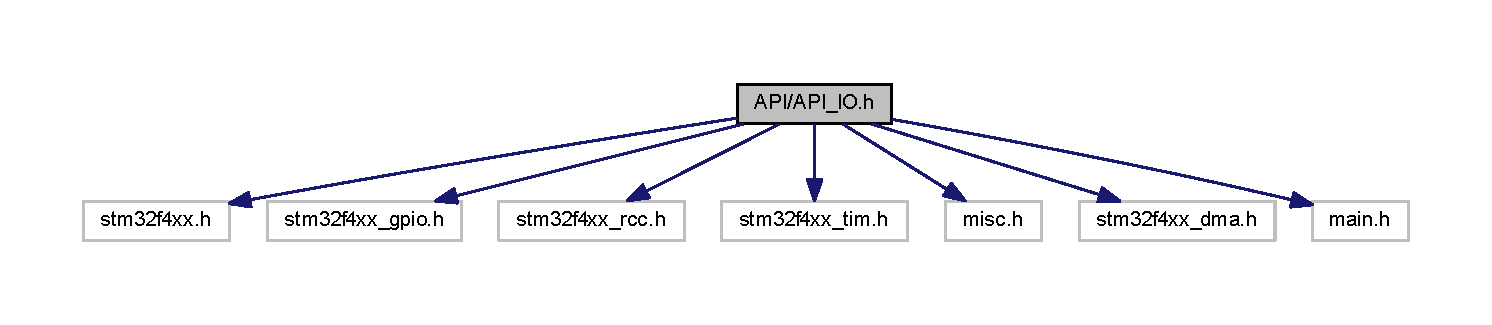
\includegraphics[width=350pt]{_a_p_i___i_o_8h__incl}
\end{center}
\end{figure}
This graph shows which files directly or indirectly include this file\+:\nopagebreak
\begin{figure}[H]
\begin{center}
\leavevmode
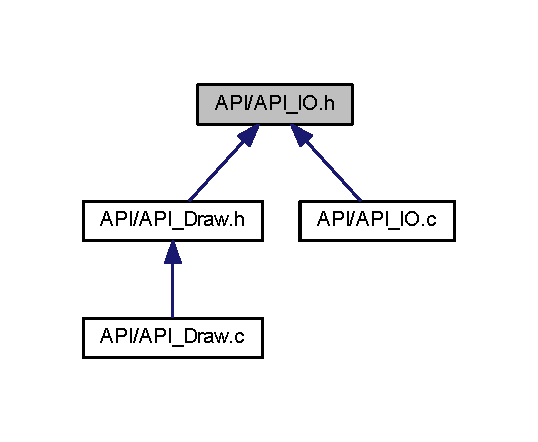
\includegraphics[width=350pt]{_a_p_i___i_o_8h__dep__incl}
\end{center}
\end{figure}
\subsection*{Data Structures}
\begin{DoxyCompactItemize}
\item 
struct \hyperlink{struct_c_o_m_m_a_n_d__t}{C\+O\+M\+M\+A\+N\+D\+\_\+t}
\begin{DoxyCompactList}\small\item\em Structure for the buffers. \end{DoxyCompactList}\item 
struct \hyperlink{struct_v_g_a__t}{V\+G\+A\+\_\+t}
\begin{DoxyCompactList}\small\item\em V\+GA structure. \end{DoxyCompactList}\end{DoxyCompactItemize}
\subsection*{Macros}
\begin{DoxyCompactItemize}
\item 
\#define \hyperlink{_a_p_i___i_o_8h_a9fee0c95dea1cdd3eeb3605ece528a8a}{V\+G\+A\+\_\+\+C\+O\+L\+\_\+\+B\+L\+A\+CK}~0x00
\begin{DoxyCompactList}\small\item\em Pixel color black. \end{DoxyCompactList}\item 
\#define \hyperlink{_a_p_i___i_o_8h_a5c55e697abe70bd280e9ce5059ff6370}{V\+G\+A\+\_\+\+C\+O\+L\+\_\+\+B\+R\+O\+WN}~0x88
\begin{DoxyCompactList}\small\item\em Pixel color brown. \end{DoxyCompactList}\item 
\#define \hyperlink{_a_p_i___i_o_8h_a9314f832988df57045bf9790f18de6fa}{V\+G\+A\+\_\+\+C\+O\+L\+\_\+\+B\+L\+UE}~0x03
\begin{DoxyCompactList}\small\item\em Pixel color blue. \end{DoxyCompactList}\item 
\#define \hyperlink{_a_p_i___i_o_8h_a28ba4fa390cd2588f7eda1cb00d251ce}{V\+G\+A\+\_\+\+C\+O\+L\+\_\+\+L\+I\+G\+H\+T\+\_\+\+B\+L\+UE}~0x6F
\begin{DoxyCompactList}\small\item\em Pixel color light blue. \end{DoxyCompactList}\item 
\#define \hyperlink{_a_p_i___i_o_8h_a4d6fe9b05dffe892c693d6cbdb3bdc94}{V\+G\+A\+\_\+\+C\+O\+L\+\_\+\+G\+R\+AY}~0x92
\begin{DoxyCompactList}\small\item\em Pixel color gray. \end{DoxyCompactList}\item 
\#define \hyperlink{_a_p_i___i_o_8h_acd643373461ea57a495e8403ba41eab7}{V\+G\+A\+\_\+\+C\+O\+L\+\_\+\+G\+R\+E\+EN}~0x1C
\begin{DoxyCompactList}\small\item\em Pixel color green. \end{DoxyCompactList}\item 
\#define \hyperlink{_a_p_i___i_o_8h_adb3602cba63f07477507c54a540d52a9}{V\+G\+A\+\_\+\+C\+O\+L\+\_\+\+L\+I\+G\+H\+T\+\_\+\+G\+R\+E\+EN}~0x7E
\begin{DoxyCompactList}\small\item\em Pixel color light green. \end{DoxyCompactList}\item 
\#define \hyperlink{_a_p_i___i_o_8h_a790cc430619a64faf356c303f8bdd3d4}{V\+G\+A\+\_\+\+C\+O\+L\+\_\+\+R\+ED}~0x\+E0
\begin{DoxyCompactList}\small\item\em Pixel color red. \end{DoxyCompactList}\item 
\#define \hyperlink{_a_p_i___i_o_8h_ae6a3ce91f16bab22b2c56fd41dccf1ea}{V\+G\+A\+\_\+\+C\+O\+L\+\_\+\+L\+I\+G\+H\+T\+\_\+\+R\+ED}~0x\+F2
\begin{DoxyCompactList}\small\item\em Pixel color light red. \end{DoxyCompactList}\item 
\#define \hyperlink{_a_p_i___i_o_8h_a2ad592a88539ed90dd1fe6c33648a13b}{V\+G\+A\+\_\+\+C\+O\+L\+\_\+\+W\+H\+I\+TE}~0x\+FF
\begin{DoxyCompactList}\small\item\em Pixel white. \end{DoxyCompactList}\item 
\#define \hyperlink{_a_p_i___i_o_8h_a39a87dbbf6639be1a1312dbe9229c4a8}{V\+G\+A\+\_\+\+C\+O\+L\+\_\+\+C\+Y\+AN}~0x1F
\begin{DoxyCompactList}\small\item\em Pixel color cyan. \end{DoxyCompactList}\item 
\#define \hyperlink{_a_p_i___i_o_8h_af1696722e55ba25438cec5c53d2eddb3}{V\+G\+A\+\_\+\+C\+O\+L\+\_\+\+L\+I\+G\+H\+T\+\_\+\+C\+Y\+AN}~0x9F
\begin{DoxyCompactList}\small\item\em Pixel light cyan. \end{DoxyCompactList}\item 
\#define \hyperlink{_a_p_i___i_o_8h_a9498759c02ab7d643c9af53a70d15ad5}{V\+G\+A\+\_\+\+C\+O\+L\+\_\+\+M\+A\+G\+E\+N\+TA}~0x\+E3
\begin{DoxyCompactList}\small\item\em Pixel magenta. \end{DoxyCompactList}\item 
\#define \hyperlink{_a_p_i___i_o_8h_ae34663271c91b95a34d721a24e0f1c1e}{V\+G\+A\+\_\+\+C\+O\+L\+\_\+\+L\+I\+G\+H\+T\+\_\+\+M\+A\+G\+E\+N\+TA}~0x\+F3
\begin{DoxyCompactList}\small\item\em Pixel light magenta. \end{DoxyCompactList}\item 
\#define \hyperlink{_a_p_i___i_o_8h_a76575b7810719497e2b15a6709c1b6f0}{V\+G\+A\+\_\+\+C\+O\+L\+\_\+\+Y\+E\+L\+L\+OW}~0x\+FC
\begin{DoxyCompactList}\small\item\em Pixel color yellow. \end{DoxyCompactList}\item 
\#define \hyperlink{_a_p_i___i_o_8h_ace7f348dc91111917772d3e19f8821d3}{V\+G\+A\+\_\+\+D\+I\+S\+P\+L\+A\+Y\+\_\+X}~320
\item 
\#define \hyperlink{_a_p_i___i_o_8h_a9c3e46882b624fe1887d0ec6171d771b}{V\+G\+A\+\_\+\+D\+I\+S\+P\+L\+A\+Y\+\_\+Y}~240
\item 
\#define \hyperlink{_a_p_i___i_o_8h_a9e8aaf9c28f704136d8fc1ba043b6bf5}{S\+T\+R\+\_\+\+L\+E\+N\+G\+TH}~120
\item 
\#define \hyperlink{_a_p_i___i_o_8h_a7be6924e0d85f3f82149ea31cca36887}{T\+Y\+P\+E\+\_\+\+L\+E\+N\+G\+TH}~20
\item 
\#define \hyperlink{_a_p_i___i_o_8h_af84c4272cc109cfaf6ed2f2000cb2904}{C\+O\+L\+O\+R\+\_\+\+L\+E\+N\+G\+TH}~20
\item 
\#define \hyperlink{_a_p_i___i_o_8h_ae833776b4ba8fc4f5d81b239fc856553}{C\+R\+C\+H\+AR}~13
\item 
\#define \hyperlink{_a_p_i___i_o_8h_a994c6410d36b46eb164dfcb0fcb82d0d}{L\+F\+C\+H\+AR}~10
\item 
\mbox{\Hypertarget{_a_p_i___i_o_8h_a9934465d996215f7e3a39f574116cd16}\label{_a_p_i___i_o_8h_a9934465d996215f7e3a39f574116cd16}} 
\#define {\bfseries V\+G\+A\+\_\+\+T\+I\+M1\+\_\+\+P\+E\+R\+I\+O\+DE}~11
\item 
\mbox{\Hypertarget{_a_p_i___i_o_8h_ab20ff576649ab2c78f0f87b758c2705b}\label{_a_p_i___i_o_8h_ab20ff576649ab2c78f0f87b758c2705b}} 
\#define {\bfseries V\+G\+A\+\_\+\+T\+I\+M1\+\_\+\+P\+R\+E\+S\+C\+A\+LE}~0
\item 
\mbox{\Hypertarget{_a_p_i___i_o_8h_a6781ff356015bb423813eb349582faa3}\label{_a_p_i___i_o_8h_a6781ff356015bb423813eb349582faa3}} 
\#define {\bfseries V\+G\+A\+\_\+\+T\+I\+M2\+\_\+\+H\+S\+Y\+N\+C\+\_\+\+P\+E\+R\+I\+O\+DE}~2667
\item 
\mbox{\Hypertarget{_a_p_i___i_o_8h_ae0124ad9d53b4c2af5902820421aea02}\label{_a_p_i___i_o_8h_ae0124ad9d53b4c2af5902820421aea02}} 
\#define {\bfseries V\+G\+A\+\_\+\+T\+I\+M2\+\_\+\+H\+S\+Y\+N\+C\+\_\+\+P\+R\+E\+S\+C\+A\+LE}~0
\item 
\mbox{\Hypertarget{_a_p_i___i_o_8h_ad3ef518a75a4d574f2a36ce343157676}\label{_a_p_i___i_o_8h_ad3ef518a75a4d574f2a36ce343157676}} 
\#define {\bfseries V\+G\+A\+\_\+\+T\+I\+M2\+\_\+\+H\+S\+Y\+N\+C\+\_\+\+I\+MP}~320
\item 
\mbox{\Hypertarget{_a_p_i___i_o_8h_a5dabd74236cb9b42d94ccc7435176d40}\label{_a_p_i___i_o_8h_a5dabd74236cb9b42d94ccc7435176d40}} 
\#define {\bfseries V\+G\+A\+\_\+\+T\+I\+M2\+\_\+\+H\+T\+R\+I\+G\+G\+E\+R\+\_\+\+S\+T\+A\+RT}~480
\item 
\mbox{\Hypertarget{_a_p_i___i_o_8h_ae0447f6b6430a8c09536288b2b01abb4}\label{_a_p_i___i_o_8h_ae0447f6b6430a8c09536288b2b01abb4}} 
\#define {\bfseries V\+G\+A\+\_\+\+T\+I\+M2\+\_\+\+D\+M\+A\+\_\+\+D\+E\+L\+AY}~60
\item 
\mbox{\Hypertarget{_a_p_i___i_o_8h_a73e729af6a6a2eb20ef3804cf794e4bd}\label{_a_p_i___i_o_8h_a73e729af6a6a2eb20ef3804cf794e4bd}} 
\#define {\bfseries V\+G\+A\+\_\+\+V\+S\+Y\+N\+C\+\_\+\+P\+E\+R\+I\+O\+DE}~525
\item 
\mbox{\Hypertarget{_a_p_i___i_o_8h_ad3c951f66600690235db2c93e74bc82f}\label{_a_p_i___i_o_8h_ad3c951f66600690235db2c93e74bc82f}} 
\#define {\bfseries V\+G\+A\+\_\+\+V\+S\+Y\+N\+C\+\_\+\+I\+MP}~2
\item 
\mbox{\Hypertarget{_a_p_i___i_o_8h_a1bf220647b6ad6187cc358cbffbb74fc}\label{_a_p_i___i_o_8h_a1bf220647b6ad6187cc358cbffbb74fc}} 
\#define {\bfseries V\+G\+A\+\_\+\+V\+S\+Y\+N\+C\+\_\+\+B\+I\+L\+D\+\_\+\+S\+T\+A\+RT}~36
\item 
\mbox{\Hypertarget{_a_p_i___i_o_8h_abf14fb3313d4de9367100e2dcddcd39f}\label{_a_p_i___i_o_8h_abf14fb3313d4de9367100e2dcddcd39f}} 
\#define {\bfseries V\+G\+A\+\_\+\+V\+S\+Y\+N\+C\+\_\+\+B\+I\+L\+D\+\_\+\+S\+T\+OP}~514
\item 
\mbox{\Hypertarget{_a_p_i___i_o_8h_a758dadcf25d5a3b26f4791e9a332f1bb}\label{_a_p_i___i_o_8h_a758dadcf25d5a3b26f4791e9a332f1bb}} 
\#define {\bfseries V\+G\+A\+\_\+\+G\+P\+I\+O\+E\+\_\+\+B\+A\+S\+E\+\_\+\+A\+DR}~((uint32\+\_\+t)0x40021000)
\item 
\mbox{\Hypertarget{_a_p_i___i_o_8h_af70daf7e1e57589c259536efc1187d6c}\label{_a_p_i___i_o_8h_af70daf7e1e57589c259536efc1187d6c}} 
\#define {\bfseries V\+G\+A\+\_\+\+G\+P\+I\+O\+\_\+\+O\+D\+R\+\_\+\+O\+F\+F\+S\+ET}~((uint32\+\_\+t)0x00000014)
\item 
\mbox{\Hypertarget{_a_p_i___i_o_8h_ac3336e31bfbbd8199e506f39164a19eb}\label{_a_p_i___i_o_8h_ac3336e31bfbbd8199e506f39164a19eb}} 
\#define {\bfseries V\+G\+A\+\_\+\+G\+P\+I\+O\+\_\+\+B\+Y\+T\+E\+\_\+\+O\+F\+F\+S\+ET}~((uint32\+\_\+t)0x00000001)
\item 
\mbox{\Hypertarget{_a_p_i___i_o_8h_a2fb72da69dd330b1ebbff2b8550d1db2}\label{_a_p_i___i_o_8h_a2fb72da69dd330b1ebbff2b8550d1db2}} 
\#define {\bfseries V\+G\+A\+\_\+\+G\+P\+I\+O\+E\+\_\+\+O\+D\+R\+\_\+\+A\+D\+D\+R\+E\+SS}~(V\+G\+A\+\_\+\+G\+P\+I\+O\+E\+\_\+\+B\+A\+S\+E\+\_\+\+A\+DR $\vert$ V\+G\+A\+\_\+\+G\+P\+I\+O\+\_\+\+O\+D\+R\+\_\+\+O\+F\+F\+S\+ET $\vert$ V\+G\+A\+\_\+\+G\+P\+I\+O\+\_\+\+B\+Y\+T\+E\+\_\+\+O\+F\+F\+S\+ET)
\item 
\mbox{\Hypertarget{_a_p_i___i_o_8h_a114dc879235023dc8e6f360a6f487a6b}\label{_a_p_i___i_o_8h_a114dc879235023dc8e6f360a6f487a6b}} 
\#define {\bfseries V\+G\+A\+\_\+\+G\+P\+I\+O\+\_\+\+H\+I\+N\+I\+B\+B\+LE}~((uint16\+\_\+t)0x\+F\+F00)
\end{DoxyCompactItemize}
\subsection*{Functions}
\begin{DoxyCompactItemize}
\item 
\mbox{\Hypertarget{_a_p_i___i_o_8h_a559918a2721e31ee27be6e026e444eca}\label{_a_p_i___i_o_8h_a559918a2721e31ee27be6e026e444eca}} 
void \hyperlink{_a_p_i___i_o_8h_a559918a2721e31ee27be6e026e444eca}{A\+P\+I\+\_\+\+I\+O\+\_\+\+Screen\+\_\+\+Init} (void)
\begin{DoxyCompactList}\small\item\em Initialize V\+G\+A-\/\+Module. \end{DoxyCompactList}\item 
void \hyperlink{_a_p_i___i_o_8h_adac57ec1d2019647d4ef389972d4ad54}{A\+P\+I\+\_\+\+I\+O\+\_\+\+Fill\+Screen} (uint8\+\_\+t color)
\begin{DoxyCompactList}\small\item\em Fill the D\+MA R\+AM buffer with one color. \end{DoxyCompactList}\item 
void \hyperlink{_a_p_i___i_o_8h_afe5040b81dac0691f4a219d04fcc70f3}{A\+P\+I\+\_\+\+I\+O\+\_\+\+Set\+Pixel} (uint16\+\_\+t xp, uint16\+\_\+t yp, uint8\+\_\+t color)
\begin{DoxyCompactList}\small\item\em Sets pixels on the screen with the chosen color. \end{DoxyCompactList}\item 
\mbox{\Hypertarget{_a_p_i___i_o_8h_ae4d306e45175f38cb244c89ee5732da8}\label{_a_p_i___i_o_8h_ae4d306e45175f38cb244c89ee5732da8}} 
void \hyperlink{_a_p_i___i_o_8h_ae4d306e45175f38cb244c89ee5732da8}{A\+P\+I\+\_\+\+I\+O\+\_\+\+Delay\+\_\+\+Init} (void)
\begin{DoxyCompactList}\small\item\em Initialize Delay. \end{DoxyCompactList}\item 
\mbox{\Hypertarget{_a_p_i___i_o_8h_ae814d208edb978c2ac0efcdfefb2e15d}\label{_a_p_i___i_o_8h_ae814d208edb978c2ac0efcdfefb2e15d}} 
void \hyperlink{_a_p_i___i_o_8h_ae814d208edb978c2ac0efcdfefb2e15d}{A\+P\+I\+\_\+\+I\+O\+\_\+\+Delay\+Micros} (uint32\+\_\+t micros)
\begin{DoxyCompactList}\small\item\em Delays in microseconds. \end{DoxyCompactList}\item 
\mbox{\Hypertarget{_a_p_i___i_o_8h_a26b3c2d0a1161d9e1dc1a15355ba5c71}\label{_a_p_i___i_o_8h_a26b3c2d0a1161d9e1dc1a15355ba5c71}} 
void \hyperlink{_a_p_i___i_o_8h_a26b3c2d0a1161d9e1dc1a15355ba5c71}{A\+P\+I\+\_\+\+I\+O\+\_\+\+Delay\+Millis} (uint32\+\_\+t millis)
\begin{DoxyCompactList}\small\item\em Delays in milliseconds. \end{DoxyCompactList}\item 
\mbox{\Hypertarget{_a_p_i___i_o_8h_a143471ba66072b8c06e360b6e91a4eb8}\label{_a_p_i___i_o_8h_a143471ba66072b8c06e360b6e91a4eb8}} 
void \hyperlink{_a_p_i___i_o_8h_a143471ba66072b8c06e360b6e91a4eb8}{A\+P\+I\+\_\+\+I\+O\+\_\+\+U\+A\+R\+T\+\_\+init} (void)
\begin{DoxyCompactList}\small\item\em Initialize the U\+A\+RT. \end{DoxyCompactList}\item 
\mbox{\Hypertarget{_a_p_i___i_o_8h_acb304b4dece8bc84d4d6eeae4961574a}\label{_a_p_i___i_o_8h_acb304b4dece8bc84d4d6eeae4961574a}} 
void \hyperlink{_a_p_i___i_o_8h_acb304b4dece8bc84d4d6eeae4961574a}{A\+P\+I\+\_\+\+I\+O\+\_\+\+U\+A\+R\+T\+\_\+\+I\+N\+T\+\_\+init} (void)
\begin{DoxyCompactList}\small\item\em Initialize the U\+A\+RT interrupt. \end{DoxyCompactList}\item 
\mbox{\Hypertarget{_a_p_i___i_o_8h_a96affedb9de9e40ef68933433b0e47a4}\label{_a_p_i___i_o_8h_a96affedb9de9e40ef68933433b0e47a4}} 
void \hyperlink{_a_p_i___i_o_8h_a96affedb9de9e40ef68933433b0e47a4}{A\+P\+I\+\_\+\+I\+O\+\_\+\+U\+A\+R\+T\+\_\+putchar} (char c)
\begin{DoxyCompactList}\small\item\em U\+A\+RT writes a char \mbox{[}in\mbox{]} c the char that has to be put. \end{DoxyCompactList}\item 
\mbox{\Hypertarget{_a_p_i___i_o_8h_ac3d5711ccd089f4195b3885195de3926}\label{_a_p_i___i_o_8h_ac3d5711ccd089f4195b3885195de3926}} 
void \hyperlink{_a_p_i___i_o_8h_ac3d5711ccd089f4195b3885195de3926}{A\+P\+I\+\_\+\+I\+O\+\_\+\+U\+A\+R\+T\+\_\+puts} (char $\ast$s)
\begin{DoxyCompactList}\small\item\em U\+A\+RT writes a string \mbox{[}in\mbox{]} s the string that has to be put. \end{DoxyCompactList}\item 
\mbox{\Hypertarget{_a_p_i___i_o_8h_a388c5d59e3272951cb0dc0105fbc5c14}\label{_a_p_i___i_o_8h_a388c5d59e3272951cb0dc0105fbc5c14}} 
void \hyperlink{_a_p_i___i_o_8h_a388c5d59e3272951cb0dc0105fbc5c14}{A\+P\+I\+\_\+\+I\+O\+\_\+\+U\+A\+R\+T\+\_\+putnum} (unsigned int num, unsigned char deel)
\begin{DoxyCompactList}\small\item\em U\+A\+RT writes an unsigned in given number system \mbox{[}in\mbox{]} num the integer that has to be put \mbox{[}in\mbox{]} deel the number system in which the integer has to put. \end{DoxyCompactList}\item 
\mbox{\Hypertarget{_a_p_i___i_o_8h_a2df6bc692c5795a4942485f9182c0250}\label{_a_p_i___i_o_8h_a2df6bc692c5795a4942485f9182c0250}} 
void \hyperlink{_a_p_i___i_o_8h_a2df6bc692c5795a4942485f9182c0250}{A\+P\+I\+\_\+\+I\+O\+\_\+\+U\+A\+R\+T\+\_\+putint} (unsigned int num)
\begin{DoxyCompactList}\small\item\em U\+A\+RT writes an unsigned integer \mbox{[}in\mbox{]} num the integer that has to be put. \end{DoxyCompactList}\item 
\mbox{\Hypertarget{_a_p_i___i_o_8h_a533091814b5b2f1065249b7ddb9c4550}\label{_a_p_i___i_o_8h_a533091814b5b2f1065249b7ddb9c4550}} 
char \hyperlink{_a_p_i___i_o_8h_a533091814b5b2f1065249b7ddb9c4550}{A\+P\+I\+\_\+\+I\+O\+\_\+\+U\+A\+R\+T\+\_\+get} (void)
\begin{DoxyCompactList}\small\item\em U\+A\+RT receives incoming char. \end{DoxyCompactList}\item 
\mbox{\Hypertarget{_a_p_i___i_o_8h_a2b3b649f12bf7414f4328c51f5ab11db}\label{_a_p_i___i_o_8h_a2b3b649f12bf7414f4328c51f5ab11db}} 
void \hyperlink{_a_p_i___i_o_8h_a2b3b649f12bf7414f4328c51f5ab11db}{A\+P\+I\+\_\+\+I\+O\+\_\+\+U\+A\+R\+T\+\_\+gets} (char $\ast$s, int echo)
\begin{DoxyCompactList}\small\item\em U\+A\+RT receives incoming string \mbox{[}in\mbox{]} s string that is received \mbox{[}in\mbox{]} echo when True, send read-\/char to U\+A\+RT. \end{DoxyCompactList}\end{DoxyCompactItemize}
\subsection*{Variables}
\begin{DoxyCompactItemize}
\item 
\mbox{\Hypertarget{_a_p_i___i_o_8h_a0642526bfd4eb59d888572150ee3032a}\label{_a_p_i___i_o_8h_a0642526bfd4eb59d888572150ee3032a}} 
\hyperlink{struct_v_g_a__t}{V\+G\+A\+\_\+t} {\bfseries V\+GA}
\item 
\mbox{\Hypertarget{_a_p_i___i_o_8h_adad76feab97da661d4015659c7a7f9a8}\label{_a_p_i___i_o_8h_adad76feab97da661d4015659c7a7f9a8}} 
uint8\+\_\+t {\bfseries V\+G\+A\+\_\+\+R\+A\+M1} \mbox{[}(\hyperlink{_a_p_i___i_o_8h_ace7f348dc91111917772d3e19f8821d3}{V\+G\+A\+\_\+\+D\+I\+S\+P\+L\+A\+Y\+\_\+X}+1) $\ast$\hyperlink{_a_p_i___i_o_8h_a9c3e46882b624fe1887d0ec6171d771b}{V\+G\+A\+\_\+\+D\+I\+S\+P\+L\+A\+Y\+\_\+Y}\mbox{]}
\end{DoxyCompactItemize}


\subsection{Detailed Description}
Common definition used by all files and public A\+PI. 



\subsection{Macro Definition Documentation}
\mbox{\Hypertarget{_a_p_i___i_o_8h_af84c4272cc109cfaf6ed2f2000cb2904}\label{_a_p_i___i_o_8h_af84c4272cc109cfaf6ed2f2000cb2904}} 
\index{A\+P\+I\+\_\+\+I\+O.\+h@{A\+P\+I\+\_\+\+I\+O.\+h}!C\+O\+L\+O\+R\+\_\+\+L\+E\+N\+G\+TH@{C\+O\+L\+O\+R\+\_\+\+L\+E\+N\+G\+TH}}
\index{C\+O\+L\+O\+R\+\_\+\+L\+E\+N\+G\+TH@{C\+O\+L\+O\+R\+\_\+\+L\+E\+N\+G\+TH}!A\+P\+I\+\_\+\+I\+O.\+h@{A\+P\+I\+\_\+\+I\+O.\+h}}
\subsubsection{\texorpdfstring{C\+O\+L\+O\+R\+\_\+\+L\+E\+N\+G\+TH}{COLOR\_LENGTH}}
{\footnotesize\ttfamily \#define C\+O\+L\+O\+R\+\_\+\+L\+E\+N\+G\+TH~20}

Size of the color buffer 

Definition at line 197 of file A\+P\+I\+\_\+\+I\+O.\+h.

\mbox{\Hypertarget{_a_p_i___i_o_8h_ae833776b4ba8fc4f5d81b239fc856553}\label{_a_p_i___i_o_8h_ae833776b4ba8fc4f5d81b239fc856553}} 
\index{A\+P\+I\+\_\+\+I\+O.\+h@{A\+P\+I\+\_\+\+I\+O.\+h}!C\+R\+C\+H\+AR@{C\+R\+C\+H\+AR}}
\index{C\+R\+C\+H\+AR@{C\+R\+C\+H\+AR}!A\+P\+I\+\_\+\+I\+O.\+h@{A\+P\+I\+\_\+\+I\+O.\+h}}
\subsubsection{\texorpdfstring{C\+R\+C\+H\+AR}{CRCHAR}}
{\footnotesize\ttfamily \#define C\+R\+C\+H\+AR~13}

Value of the carriage return char 

Definition at line 202 of file A\+P\+I\+\_\+\+I\+O.\+h.

\mbox{\Hypertarget{_a_p_i___i_o_8h_a994c6410d36b46eb164dfcb0fcb82d0d}\label{_a_p_i___i_o_8h_a994c6410d36b46eb164dfcb0fcb82d0d}} 
\index{A\+P\+I\+\_\+\+I\+O.\+h@{A\+P\+I\+\_\+\+I\+O.\+h}!L\+F\+C\+H\+AR@{L\+F\+C\+H\+AR}}
\index{L\+F\+C\+H\+AR@{L\+F\+C\+H\+AR}!A\+P\+I\+\_\+\+I\+O.\+h@{A\+P\+I\+\_\+\+I\+O.\+h}}
\subsubsection{\texorpdfstring{L\+F\+C\+H\+AR}{LFCHAR}}
{\footnotesize\ttfamily \#define L\+F\+C\+H\+AR~10}

Value of the linefeed char 

Definition at line 207 of file A\+P\+I\+\_\+\+I\+O.\+h.

\mbox{\Hypertarget{_a_p_i___i_o_8h_a9e8aaf9c28f704136d8fc1ba043b6bf5}\label{_a_p_i___i_o_8h_a9e8aaf9c28f704136d8fc1ba043b6bf5}} 
\index{A\+P\+I\+\_\+\+I\+O.\+h@{A\+P\+I\+\_\+\+I\+O.\+h}!S\+T\+R\+\_\+\+L\+E\+N\+G\+TH@{S\+T\+R\+\_\+\+L\+E\+N\+G\+TH}}
\index{S\+T\+R\+\_\+\+L\+E\+N\+G\+TH@{S\+T\+R\+\_\+\+L\+E\+N\+G\+TH}!A\+P\+I\+\_\+\+I\+O.\+h@{A\+P\+I\+\_\+\+I\+O.\+h}}
\subsubsection{\texorpdfstring{S\+T\+R\+\_\+\+L\+E\+N\+G\+TH}{STR\_LENGTH}}
{\footnotesize\ttfamily \#define S\+T\+R\+\_\+\+L\+E\+N\+G\+TH~120}

Size (string length) of the fill buffer 

Definition at line 187 of file A\+P\+I\+\_\+\+I\+O.\+h.

\mbox{\Hypertarget{_a_p_i___i_o_8h_a7be6924e0d85f3f82149ea31cca36887}\label{_a_p_i___i_o_8h_a7be6924e0d85f3f82149ea31cca36887}} 
\index{A\+P\+I\+\_\+\+I\+O.\+h@{A\+P\+I\+\_\+\+I\+O.\+h}!T\+Y\+P\+E\+\_\+\+L\+E\+N\+G\+TH@{T\+Y\+P\+E\+\_\+\+L\+E\+N\+G\+TH}}
\index{T\+Y\+P\+E\+\_\+\+L\+E\+N\+G\+TH@{T\+Y\+P\+E\+\_\+\+L\+E\+N\+G\+TH}!A\+P\+I\+\_\+\+I\+O.\+h@{A\+P\+I\+\_\+\+I\+O.\+h}}
\subsubsection{\texorpdfstring{T\+Y\+P\+E\+\_\+\+L\+E\+N\+G\+TH}{TYPE\_LENGTH}}
{\footnotesize\ttfamily \#define T\+Y\+P\+E\+\_\+\+L\+E\+N\+G\+TH~20}

Size of the type buffer 

Definition at line 192 of file A\+P\+I\+\_\+\+I\+O.\+h.

\mbox{\Hypertarget{_a_p_i___i_o_8h_a9fee0c95dea1cdd3eeb3605ece528a8a}\label{_a_p_i___i_o_8h_a9fee0c95dea1cdd3eeb3605ece528a8a}} 
\index{A\+P\+I\+\_\+\+I\+O.\+h@{A\+P\+I\+\_\+\+I\+O.\+h}!V\+G\+A\+\_\+\+C\+O\+L\+\_\+\+B\+L\+A\+CK@{V\+G\+A\+\_\+\+C\+O\+L\+\_\+\+B\+L\+A\+CK}}
\index{V\+G\+A\+\_\+\+C\+O\+L\+\_\+\+B\+L\+A\+CK@{V\+G\+A\+\_\+\+C\+O\+L\+\_\+\+B\+L\+A\+CK}!A\+P\+I\+\_\+\+I\+O.\+h@{A\+P\+I\+\_\+\+I\+O.\+h}}
\subsubsection{\texorpdfstring{V\+G\+A\+\_\+\+C\+O\+L\+\_\+\+B\+L\+A\+CK}{VGA\_COL\_BLACK}}
{\footnotesize\ttfamily \#define V\+G\+A\+\_\+\+C\+O\+L\+\_\+\+B\+L\+A\+CK~0x00}



Pixel color black. 

The color value for a single pixel is stored in an 8-\/bit unsigned integer. The \doxytablelink{_a_p_i___i_o_8h_color_designation}{color\+\_\+designation} table specified how the three, red, green, and blue, colors are stored.

\hypertarget{_a_p_i___i_o_8h_color_designation}{}
\tabulinesep=1mm
\begin{longtabu} spread 0pt [c]{*{9}{|X[-1]}|}
\caption{Color Designation}\label{_a_p_i___i_o_8h_color_designation}\\
\hline
\textbf{ Bit number }&7 &6 &5 &4 &3 &2 &1 &0  \\\cline{1-9}
{\bfseries Color} &\multicolumn{3}{p{(\linewidth-\tabcolsep*9-\arrayrulewidth*4)*3/9}|}{\PBS\centering Red }&\multicolumn{3}{p{(\linewidth-\tabcolsep*9-\arrayrulewidth*4)*3/9}|}{\PBS\centering Green }&\multicolumn{2}{p{(\linewidth-\tabcolsep*9-\arrayrulewidth*4)*2/9}|}{\PBS\centering Blue  }\\\cline{1-9}
\end{longtabu}


Definition at line 60 of file A\+P\+I\+\_\+\+I\+O.\+h.

\mbox{\Hypertarget{_a_p_i___i_o_8h_a9314f832988df57045bf9790f18de6fa}\label{_a_p_i___i_o_8h_a9314f832988df57045bf9790f18de6fa}} 
\index{A\+P\+I\+\_\+\+I\+O.\+h@{A\+P\+I\+\_\+\+I\+O.\+h}!V\+G\+A\+\_\+\+C\+O\+L\+\_\+\+B\+L\+UE@{V\+G\+A\+\_\+\+C\+O\+L\+\_\+\+B\+L\+UE}}
\index{V\+G\+A\+\_\+\+C\+O\+L\+\_\+\+B\+L\+UE@{V\+G\+A\+\_\+\+C\+O\+L\+\_\+\+B\+L\+UE}!A\+P\+I\+\_\+\+I\+O.\+h@{A\+P\+I\+\_\+\+I\+O.\+h}}
\subsubsection{\texorpdfstring{V\+G\+A\+\_\+\+C\+O\+L\+\_\+\+B\+L\+UE}{VGA\_COL\_BLUE}}
{\footnotesize\ttfamily \#define V\+G\+A\+\_\+\+C\+O\+L\+\_\+\+B\+L\+UE~0x03}



Pixel color blue. 

\begin{DoxySeeAlso}{See also}
\hyperlink{_a_p_i___i_o_8h_a9fee0c95dea1cdd3eeb3605ece528a8a}{V\+G\+A\+\_\+\+C\+O\+L\+\_\+\+B\+L\+A\+CK} for a description on how the color for a single pixel is stored. 
\end{DoxySeeAlso}


Definition at line 76 of file A\+P\+I\+\_\+\+I\+O.\+h.

\mbox{\Hypertarget{_a_p_i___i_o_8h_a5c55e697abe70bd280e9ce5059ff6370}\label{_a_p_i___i_o_8h_a5c55e697abe70bd280e9ce5059ff6370}} 
\index{A\+P\+I\+\_\+\+I\+O.\+h@{A\+P\+I\+\_\+\+I\+O.\+h}!V\+G\+A\+\_\+\+C\+O\+L\+\_\+\+B\+R\+O\+WN@{V\+G\+A\+\_\+\+C\+O\+L\+\_\+\+B\+R\+O\+WN}}
\index{V\+G\+A\+\_\+\+C\+O\+L\+\_\+\+B\+R\+O\+WN@{V\+G\+A\+\_\+\+C\+O\+L\+\_\+\+B\+R\+O\+WN}!A\+P\+I\+\_\+\+I\+O.\+h@{A\+P\+I\+\_\+\+I\+O.\+h}}
\subsubsection{\texorpdfstring{V\+G\+A\+\_\+\+C\+O\+L\+\_\+\+B\+R\+O\+WN}{VGA\_COL\_BROWN}}
{\footnotesize\ttfamily \#define V\+G\+A\+\_\+\+C\+O\+L\+\_\+\+B\+R\+O\+WN~0x88}



Pixel color brown. 

\begin{DoxySeeAlso}{See also}
\hyperlink{_a_p_i___i_o_8h_a9fee0c95dea1cdd3eeb3605ece528a8a}{V\+G\+A\+\_\+\+C\+O\+L\+\_\+\+B\+L\+A\+CK} for a description on how the color for a single pixel is stored. 
\end{DoxySeeAlso}


Definition at line 68 of file A\+P\+I\+\_\+\+I\+O.\+h.

\mbox{\Hypertarget{_a_p_i___i_o_8h_a39a87dbbf6639be1a1312dbe9229c4a8}\label{_a_p_i___i_o_8h_a39a87dbbf6639be1a1312dbe9229c4a8}} 
\index{A\+P\+I\+\_\+\+I\+O.\+h@{A\+P\+I\+\_\+\+I\+O.\+h}!V\+G\+A\+\_\+\+C\+O\+L\+\_\+\+C\+Y\+AN@{V\+G\+A\+\_\+\+C\+O\+L\+\_\+\+C\+Y\+AN}}
\index{V\+G\+A\+\_\+\+C\+O\+L\+\_\+\+C\+Y\+AN@{V\+G\+A\+\_\+\+C\+O\+L\+\_\+\+C\+Y\+AN}!A\+P\+I\+\_\+\+I\+O.\+h@{A\+P\+I\+\_\+\+I\+O.\+h}}
\subsubsection{\texorpdfstring{V\+G\+A\+\_\+\+C\+O\+L\+\_\+\+C\+Y\+AN}{VGA\_COL\_CYAN}}
{\footnotesize\ttfamily \#define V\+G\+A\+\_\+\+C\+O\+L\+\_\+\+C\+Y\+AN~0x1F}



Pixel color cyan. 

\begin{DoxySeeAlso}{See also}
\hyperlink{_a_p_i___i_o_8h_a9fee0c95dea1cdd3eeb3605ece528a8a}{V\+G\+A\+\_\+\+C\+O\+L\+\_\+\+B\+L\+A\+CK} for a description on how the color for a single pixel is stored. 
\end{DoxySeeAlso}


Definition at line 140 of file A\+P\+I\+\_\+\+I\+O.\+h.

\mbox{\Hypertarget{_a_p_i___i_o_8h_a4d6fe9b05dffe892c693d6cbdb3bdc94}\label{_a_p_i___i_o_8h_a4d6fe9b05dffe892c693d6cbdb3bdc94}} 
\index{A\+P\+I\+\_\+\+I\+O.\+h@{A\+P\+I\+\_\+\+I\+O.\+h}!V\+G\+A\+\_\+\+C\+O\+L\+\_\+\+G\+R\+AY@{V\+G\+A\+\_\+\+C\+O\+L\+\_\+\+G\+R\+AY}}
\index{V\+G\+A\+\_\+\+C\+O\+L\+\_\+\+G\+R\+AY@{V\+G\+A\+\_\+\+C\+O\+L\+\_\+\+G\+R\+AY}!A\+P\+I\+\_\+\+I\+O.\+h@{A\+P\+I\+\_\+\+I\+O.\+h}}
\subsubsection{\texorpdfstring{V\+G\+A\+\_\+\+C\+O\+L\+\_\+\+G\+R\+AY}{VGA\_COL\_GRAY}}
{\footnotesize\ttfamily \#define V\+G\+A\+\_\+\+C\+O\+L\+\_\+\+G\+R\+AY~0x92}



Pixel color gray. 

\begin{DoxySeeAlso}{See also}
\hyperlink{_a_p_i___i_o_8h_a9fee0c95dea1cdd3eeb3605ece528a8a}{V\+G\+A\+\_\+\+C\+O\+L\+\_\+\+B\+L\+A\+CK} for a description on how the color for a single pixel is stored. 
\end{DoxySeeAlso}


Definition at line 92 of file A\+P\+I\+\_\+\+I\+O.\+h.

\mbox{\Hypertarget{_a_p_i___i_o_8h_acd643373461ea57a495e8403ba41eab7}\label{_a_p_i___i_o_8h_acd643373461ea57a495e8403ba41eab7}} 
\index{A\+P\+I\+\_\+\+I\+O.\+h@{A\+P\+I\+\_\+\+I\+O.\+h}!V\+G\+A\+\_\+\+C\+O\+L\+\_\+\+G\+R\+E\+EN@{V\+G\+A\+\_\+\+C\+O\+L\+\_\+\+G\+R\+E\+EN}}
\index{V\+G\+A\+\_\+\+C\+O\+L\+\_\+\+G\+R\+E\+EN@{V\+G\+A\+\_\+\+C\+O\+L\+\_\+\+G\+R\+E\+EN}!A\+P\+I\+\_\+\+I\+O.\+h@{A\+P\+I\+\_\+\+I\+O.\+h}}
\subsubsection{\texorpdfstring{V\+G\+A\+\_\+\+C\+O\+L\+\_\+\+G\+R\+E\+EN}{VGA\_COL\_GREEN}}
{\footnotesize\ttfamily \#define V\+G\+A\+\_\+\+C\+O\+L\+\_\+\+G\+R\+E\+EN~0x1C}



Pixel color green. 

\begin{DoxySeeAlso}{See also}
\hyperlink{_a_p_i___i_o_8h_a9fee0c95dea1cdd3eeb3605ece528a8a}{V\+G\+A\+\_\+\+C\+O\+L\+\_\+\+B\+L\+A\+CK} for a description on how the color for a single pixel is stored. 
\end{DoxySeeAlso}


Definition at line 100 of file A\+P\+I\+\_\+\+I\+O.\+h.

\mbox{\Hypertarget{_a_p_i___i_o_8h_a28ba4fa390cd2588f7eda1cb00d251ce}\label{_a_p_i___i_o_8h_a28ba4fa390cd2588f7eda1cb00d251ce}} 
\index{A\+P\+I\+\_\+\+I\+O.\+h@{A\+P\+I\+\_\+\+I\+O.\+h}!V\+G\+A\+\_\+\+C\+O\+L\+\_\+\+L\+I\+G\+H\+T\+\_\+\+B\+L\+UE@{V\+G\+A\+\_\+\+C\+O\+L\+\_\+\+L\+I\+G\+H\+T\+\_\+\+B\+L\+UE}}
\index{V\+G\+A\+\_\+\+C\+O\+L\+\_\+\+L\+I\+G\+H\+T\+\_\+\+B\+L\+UE@{V\+G\+A\+\_\+\+C\+O\+L\+\_\+\+L\+I\+G\+H\+T\+\_\+\+B\+L\+UE}!A\+P\+I\+\_\+\+I\+O.\+h@{A\+P\+I\+\_\+\+I\+O.\+h}}
\subsubsection{\texorpdfstring{V\+G\+A\+\_\+\+C\+O\+L\+\_\+\+L\+I\+G\+H\+T\+\_\+\+B\+L\+UE}{VGA\_COL\_LIGHT\_BLUE}}
{\footnotesize\ttfamily \#define V\+G\+A\+\_\+\+C\+O\+L\+\_\+\+L\+I\+G\+H\+T\+\_\+\+B\+L\+UE~0x6F}



Pixel color light blue. 

\begin{DoxySeeAlso}{See also}
\hyperlink{_a_p_i___i_o_8h_a9fee0c95dea1cdd3eeb3605ece528a8a}{V\+G\+A\+\_\+\+C\+O\+L\+\_\+\+B\+L\+A\+CK} for a description on how the color for a single pixel is stored. 
\end{DoxySeeAlso}


Definition at line 84 of file A\+P\+I\+\_\+\+I\+O.\+h.

\mbox{\Hypertarget{_a_p_i___i_o_8h_af1696722e55ba25438cec5c53d2eddb3}\label{_a_p_i___i_o_8h_af1696722e55ba25438cec5c53d2eddb3}} 
\index{A\+P\+I\+\_\+\+I\+O.\+h@{A\+P\+I\+\_\+\+I\+O.\+h}!V\+G\+A\+\_\+\+C\+O\+L\+\_\+\+L\+I\+G\+H\+T\+\_\+\+C\+Y\+AN@{V\+G\+A\+\_\+\+C\+O\+L\+\_\+\+L\+I\+G\+H\+T\+\_\+\+C\+Y\+AN}}
\index{V\+G\+A\+\_\+\+C\+O\+L\+\_\+\+L\+I\+G\+H\+T\+\_\+\+C\+Y\+AN@{V\+G\+A\+\_\+\+C\+O\+L\+\_\+\+L\+I\+G\+H\+T\+\_\+\+C\+Y\+AN}!A\+P\+I\+\_\+\+I\+O.\+h@{A\+P\+I\+\_\+\+I\+O.\+h}}
\subsubsection{\texorpdfstring{V\+G\+A\+\_\+\+C\+O\+L\+\_\+\+L\+I\+G\+H\+T\+\_\+\+C\+Y\+AN}{VGA\_COL\_LIGHT\_CYAN}}
{\footnotesize\ttfamily \#define V\+G\+A\+\_\+\+C\+O\+L\+\_\+\+L\+I\+G\+H\+T\+\_\+\+C\+Y\+AN~0x9F}



Pixel light cyan. 

\begin{DoxySeeAlso}{See also}
\hyperlink{_a_p_i___i_o_8h_a9fee0c95dea1cdd3eeb3605ece528a8a}{V\+G\+A\+\_\+\+C\+O\+L\+\_\+\+B\+L\+A\+CK} for a description on how the color for a single pixel is stored. 
\end{DoxySeeAlso}


Definition at line 148 of file A\+P\+I\+\_\+\+I\+O.\+h.

\mbox{\Hypertarget{_a_p_i___i_o_8h_adb3602cba63f07477507c54a540d52a9}\label{_a_p_i___i_o_8h_adb3602cba63f07477507c54a540d52a9}} 
\index{A\+P\+I\+\_\+\+I\+O.\+h@{A\+P\+I\+\_\+\+I\+O.\+h}!V\+G\+A\+\_\+\+C\+O\+L\+\_\+\+L\+I\+G\+H\+T\+\_\+\+G\+R\+E\+EN@{V\+G\+A\+\_\+\+C\+O\+L\+\_\+\+L\+I\+G\+H\+T\+\_\+\+G\+R\+E\+EN}}
\index{V\+G\+A\+\_\+\+C\+O\+L\+\_\+\+L\+I\+G\+H\+T\+\_\+\+G\+R\+E\+EN@{V\+G\+A\+\_\+\+C\+O\+L\+\_\+\+L\+I\+G\+H\+T\+\_\+\+G\+R\+E\+EN}!A\+P\+I\+\_\+\+I\+O.\+h@{A\+P\+I\+\_\+\+I\+O.\+h}}
\subsubsection{\texorpdfstring{V\+G\+A\+\_\+\+C\+O\+L\+\_\+\+L\+I\+G\+H\+T\+\_\+\+G\+R\+E\+EN}{VGA\_COL\_LIGHT\_GREEN}}
{\footnotesize\ttfamily \#define V\+G\+A\+\_\+\+C\+O\+L\+\_\+\+L\+I\+G\+H\+T\+\_\+\+G\+R\+E\+EN~0x7E}



Pixel color light green. 

\begin{DoxySeeAlso}{See also}
\hyperlink{_a_p_i___i_o_8h_a9fee0c95dea1cdd3eeb3605ece528a8a}{V\+G\+A\+\_\+\+C\+O\+L\+\_\+\+B\+L\+A\+CK} for a description on how the color for a single pixel is stored. 
\end{DoxySeeAlso}


Definition at line 108 of file A\+P\+I\+\_\+\+I\+O.\+h.

\mbox{\Hypertarget{_a_p_i___i_o_8h_ae34663271c91b95a34d721a24e0f1c1e}\label{_a_p_i___i_o_8h_ae34663271c91b95a34d721a24e0f1c1e}} 
\index{A\+P\+I\+\_\+\+I\+O.\+h@{A\+P\+I\+\_\+\+I\+O.\+h}!V\+G\+A\+\_\+\+C\+O\+L\+\_\+\+L\+I\+G\+H\+T\+\_\+\+M\+A\+G\+E\+N\+TA@{V\+G\+A\+\_\+\+C\+O\+L\+\_\+\+L\+I\+G\+H\+T\+\_\+\+M\+A\+G\+E\+N\+TA}}
\index{V\+G\+A\+\_\+\+C\+O\+L\+\_\+\+L\+I\+G\+H\+T\+\_\+\+M\+A\+G\+E\+N\+TA@{V\+G\+A\+\_\+\+C\+O\+L\+\_\+\+L\+I\+G\+H\+T\+\_\+\+M\+A\+G\+E\+N\+TA}!A\+P\+I\+\_\+\+I\+O.\+h@{A\+P\+I\+\_\+\+I\+O.\+h}}
\subsubsection{\texorpdfstring{V\+G\+A\+\_\+\+C\+O\+L\+\_\+\+L\+I\+G\+H\+T\+\_\+\+M\+A\+G\+E\+N\+TA}{VGA\_COL\_LIGHT\_MAGENTA}}
{\footnotesize\ttfamily \#define V\+G\+A\+\_\+\+C\+O\+L\+\_\+\+L\+I\+G\+H\+T\+\_\+\+M\+A\+G\+E\+N\+TA~0x\+F3}



Pixel light magenta. 

\begin{DoxySeeAlso}{See also}
\hyperlink{_a_p_i___i_o_8h_a9fee0c95dea1cdd3eeb3605ece528a8a}{V\+G\+A\+\_\+\+C\+O\+L\+\_\+\+B\+L\+A\+CK} for a description on how the color for a single pixel is stored. 
\end{DoxySeeAlso}


Definition at line 164 of file A\+P\+I\+\_\+\+I\+O.\+h.

\mbox{\Hypertarget{_a_p_i___i_o_8h_ae6a3ce91f16bab22b2c56fd41dccf1ea}\label{_a_p_i___i_o_8h_ae6a3ce91f16bab22b2c56fd41dccf1ea}} 
\index{A\+P\+I\+\_\+\+I\+O.\+h@{A\+P\+I\+\_\+\+I\+O.\+h}!V\+G\+A\+\_\+\+C\+O\+L\+\_\+\+L\+I\+G\+H\+T\+\_\+\+R\+ED@{V\+G\+A\+\_\+\+C\+O\+L\+\_\+\+L\+I\+G\+H\+T\+\_\+\+R\+ED}}
\index{V\+G\+A\+\_\+\+C\+O\+L\+\_\+\+L\+I\+G\+H\+T\+\_\+\+R\+ED@{V\+G\+A\+\_\+\+C\+O\+L\+\_\+\+L\+I\+G\+H\+T\+\_\+\+R\+ED}!A\+P\+I\+\_\+\+I\+O.\+h@{A\+P\+I\+\_\+\+I\+O.\+h}}
\subsubsection{\texorpdfstring{V\+G\+A\+\_\+\+C\+O\+L\+\_\+\+L\+I\+G\+H\+T\+\_\+\+R\+ED}{VGA\_COL\_LIGHT\_RED}}
{\footnotesize\ttfamily \#define V\+G\+A\+\_\+\+C\+O\+L\+\_\+\+L\+I\+G\+H\+T\+\_\+\+R\+ED~0x\+F2}



Pixel color light red. 

\begin{DoxySeeAlso}{See also}
\hyperlink{_a_p_i___i_o_8h_a9fee0c95dea1cdd3eeb3605ece528a8a}{V\+G\+A\+\_\+\+C\+O\+L\+\_\+\+B\+L\+A\+CK} for a description on how the color for a single pixel is stored. 
\end{DoxySeeAlso}


Definition at line 124 of file A\+P\+I\+\_\+\+I\+O.\+h.

\mbox{\Hypertarget{_a_p_i___i_o_8h_a9498759c02ab7d643c9af53a70d15ad5}\label{_a_p_i___i_o_8h_a9498759c02ab7d643c9af53a70d15ad5}} 
\index{A\+P\+I\+\_\+\+I\+O.\+h@{A\+P\+I\+\_\+\+I\+O.\+h}!V\+G\+A\+\_\+\+C\+O\+L\+\_\+\+M\+A\+G\+E\+N\+TA@{V\+G\+A\+\_\+\+C\+O\+L\+\_\+\+M\+A\+G\+E\+N\+TA}}
\index{V\+G\+A\+\_\+\+C\+O\+L\+\_\+\+M\+A\+G\+E\+N\+TA@{V\+G\+A\+\_\+\+C\+O\+L\+\_\+\+M\+A\+G\+E\+N\+TA}!A\+P\+I\+\_\+\+I\+O.\+h@{A\+P\+I\+\_\+\+I\+O.\+h}}
\subsubsection{\texorpdfstring{V\+G\+A\+\_\+\+C\+O\+L\+\_\+\+M\+A\+G\+E\+N\+TA}{VGA\_COL\_MAGENTA}}
{\footnotesize\ttfamily \#define V\+G\+A\+\_\+\+C\+O\+L\+\_\+\+M\+A\+G\+E\+N\+TA~0x\+E3}



Pixel magenta. 

\begin{DoxySeeAlso}{See also}
\hyperlink{_a_p_i___i_o_8h_a9fee0c95dea1cdd3eeb3605ece528a8a}{V\+G\+A\+\_\+\+C\+O\+L\+\_\+\+B\+L\+A\+CK} for a description on how the color for a single pixel is stored. 
\end{DoxySeeAlso}


Definition at line 156 of file A\+P\+I\+\_\+\+I\+O.\+h.

\mbox{\Hypertarget{_a_p_i___i_o_8h_a790cc430619a64faf356c303f8bdd3d4}\label{_a_p_i___i_o_8h_a790cc430619a64faf356c303f8bdd3d4}} 
\index{A\+P\+I\+\_\+\+I\+O.\+h@{A\+P\+I\+\_\+\+I\+O.\+h}!V\+G\+A\+\_\+\+C\+O\+L\+\_\+\+R\+ED@{V\+G\+A\+\_\+\+C\+O\+L\+\_\+\+R\+ED}}
\index{V\+G\+A\+\_\+\+C\+O\+L\+\_\+\+R\+ED@{V\+G\+A\+\_\+\+C\+O\+L\+\_\+\+R\+ED}!A\+P\+I\+\_\+\+I\+O.\+h@{A\+P\+I\+\_\+\+I\+O.\+h}}
\subsubsection{\texorpdfstring{V\+G\+A\+\_\+\+C\+O\+L\+\_\+\+R\+ED}{VGA\_COL\_RED}}
{\footnotesize\ttfamily \#define V\+G\+A\+\_\+\+C\+O\+L\+\_\+\+R\+ED~0x\+E0}



Pixel color red. 

\begin{DoxySeeAlso}{See also}
\hyperlink{_a_p_i___i_o_8h_a9fee0c95dea1cdd3eeb3605ece528a8a}{V\+G\+A\+\_\+\+C\+O\+L\+\_\+\+B\+L\+A\+CK} for a description on how the color for a single pixel is stored. 
\end{DoxySeeAlso}


Definition at line 116 of file A\+P\+I\+\_\+\+I\+O.\+h.

\mbox{\Hypertarget{_a_p_i___i_o_8h_a2ad592a88539ed90dd1fe6c33648a13b}\label{_a_p_i___i_o_8h_a2ad592a88539ed90dd1fe6c33648a13b}} 
\index{A\+P\+I\+\_\+\+I\+O.\+h@{A\+P\+I\+\_\+\+I\+O.\+h}!V\+G\+A\+\_\+\+C\+O\+L\+\_\+\+W\+H\+I\+TE@{V\+G\+A\+\_\+\+C\+O\+L\+\_\+\+W\+H\+I\+TE}}
\index{V\+G\+A\+\_\+\+C\+O\+L\+\_\+\+W\+H\+I\+TE@{V\+G\+A\+\_\+\+C\+O\+L\+\_\+\+W\+H\+I\+TE}!A\+P\+I\+\_\+\+I\+O.\+h@{A\+P\+I\+\_\+\+I\+O.\+h}}
\subsubsection{\texorpdfstring{V\+G\+A\+\_\+\+C\+O\+L\+\_\+\+W\+H\+I\+TE}{VGA\_COL\_WHITE}}
{\footnotesize\ttfamily \#define V\+G\+A\+\_\+\+C\+O\+L\+\_\+\+W\+H\+I\+TE~0x\+FF}



Pixel white. 

\begin{DoxySeeAlso}{See also}
\hyperlink{_a_p_i___i_o_8h_a9fee0c95dea1cdd3eeb3605ece528a8a}{V\+G\+A\+\_\+\+C\+O\+L\+\_\+\+B\+L\+A\+CK} for a description on how the color for a single pixel is stored. 
\end{DoxySeeAlso}


Definition at line 132 of file A\+P\+I\+\_\+\+I\+O.\+h.

\mbox{\Hypertarget{_a_p_i___i_o_8h_a76575b7810719497e2b15a6709c1b6f0}\label{_a_p_i___i_o_8h_a76575b7810719497e2b15a6709c1b6f0}} 
\index{A\+P\+I\+\_\+\+I\+O.\+h@{A\+P\+I\+\_\+\+I\+O.\+h}!V\+G\+A\+\_\+\+C\+O\+L\+\_\+\+Y\+E\+L\+L\+OW@{V\+G\+A\+\_\+\+C\+O\+L\+\_\+\+Y\+E\+L\+L\+OW}}
\index{V\+G\+A\+\_\+\+C\+O\+L\+\_\+\+Y\+E\+L\+L\+OW@{V\+G\+A\+\_\+\+C\+O\+L\+\_\+\+Y\+E\+L\+L\+OW}!A\+P\+I\+\_\+\+I\+O.\+h@{A\+P\+I\+\_\+\+I\+O.\+h}}
\subsubsection{\texorpdfstring{V\+G\+A\+\_\+\+C\+O\+L\+\_\+\+Y\+E\+L\+L\+OW}{VGA\_COL\_YELLOW}}
{\footnotesize\ttfamily \#define V\+G\+A\+\_\+\+C\+O\+L\+\_\+\+Y\+E\+L\+L\+OW~0x\+FC}



Pixel color yellow. 

\begin{DoxySeeAlso}{See also}
\hyperlink{_a_p_i___i_o_8h_a9fee0c95dea1cdd3eeb3605ece528a8a}{V\+G\+A\+\_\+\+C\+O\+L\+\_\+\+B\+L\+A\+CK} for a description on how the color for a single pixel is stored. 
\end{DoxySeeAlso}


Definition at line 172 of file A\+P\+I\+\_\+\+I\+O.\+h.

\mbox{\Hypertarget{_a_p_i___i_o_8h_ace7f348dc91111917772d3e19f8821d3}\label{_a_p_i___i_o_8h_ace7f348dc91111917772d3e19f8821d3}} 
\index{A\+P\+I\+\_\+\+I\+O.\+h@{A\+P\+I\+\_\+\+I\+O.\+h}!V\+G\+A\+\_\+\+D\+I\+S\+P\+L\+A\+Y\+\_\+X@{V\+G\+A\+\_\+\+D\+I\+S\+P\+L\+A\+Y\+\_\+X}}
\index{V\+G\+A\+\_\+\+D\+I\+S\+P\+L\+A\+Y\+\_\+X@{V\+G\+A\+\_\+\+D\+I\+S\+P\+L\+A\+Y\+\_\+X}!A\+P\+I\+\_\+\+I\+O.\+h@{A\+P\+I\+\_\+\+I\+O.\+h}}
\subsubsection{\texorpdfstring{V\+G\+A\+\_\+\+D\+I\+S\+P\+L\+A\+Y\+\_\+X}{VGA\_DISPLAY\_X}}
{\footnotesize\ttfamily \#define V\+G\+A\+\_\+\+D\+I\+S\+P\+L\+A\+Y\+\_\+X~320}

Width of the V\+GA display 

Definition at line 177 of file A\+P\+I\+\_\+\+I\+O.\+h.

\mbox{\Hypertarget{_a_p_i___i_o_8h_a9c3e46882b624fe1887d0ec6171d771b}\label{_a_p_i___i_o_8h_a9c3e46882b624fe1887d0ec6171d771b}} 
\index{A\+P\+I\+\_\+\+I\+O.\+h@{A\+P\+I\+\_\+\+I\+O.\+h}!V\+G\+A\+\_\+\+D\+I\+S\+P\+L\+A\+Y\+\_\+Y@{V\+G\+A\+\_\+\+D\+I\+S\+P\+L\+A\+Y\+\_\+Y}}
\index{V\+G\+A\+\_\+\+D\+I\+S\+P\+L\+A\+Y\+\_\+Y@{V\+G\+A\+\_\+\+D\+I\+S\+P\+L\+A\+Y\+\_\+Y}!A\+P\+I\+\_\+\+I\+O.\+h@{A\+P\+I\+\_\+\+I\+O.\+h}}
\subsubsection{\texorpdfstring{V\+G\+A\+\_\+\+D\+I\+S\+P\+L\+A\+Y\+\_\+Y}{VGA\_DISPLAY\_Y}}
{\footnotesize\ttfamily \#define V\+G\+A\+\_\+\+D\+I\+S\+P\+L\+A\+Y\+\_\+Y~240}

Height of the V\+GA display 

Definition at line 182 of file A\+P\+I\+\_\+\+I\+O.\+h.



\subsection{Function Documentation}
\mbox{\Hypertarget{_a_p_i___i_o_8h_adac57ec1d2019647d4ef389972d4ad54}\label{_a_p_i___i_o_8h_adac57ec1d2019647d4ef389972d4ad54}} 
\index{A\+P\+I\+\_\+\+I\+O.\+h@{A\+P\+I\+\_\+\+I\+O.\+h}!A\+P\+I\+\_\+\+I\+O\+\_\+\+Fill\+Screen@{A\+P\+I\+\_\+\+I\+O\+\_\+\+Fill\+Screen}}
\index{A\+P\+I\+\_\+\+I\+O\+\_\+\+Fill\+Screen@{A\+P\+I\+\_\+\+I\+O\+\_\+\+Fill\+Screen}!A\+P\+I\+\_\+\+I\+O.\+h@{A\+P\+I\+\_\+\+I\+O.\+h}}
\subsubsection{\texorpdfstring{A\+P\+I\+\_\+\+I\+O\+\_\+\+Fill\+Screen()}{API\_IO\_FillScreen()}}
{\footnotesize\ttfamily void A\+P\+I\+\_\+\+I\+O\+\_\+\+Fill\+Screen (\begin{DoxyParamCaption}\item[{uint8\+\_\+t}]{color }\end{DoxyParamCaption})}



Fill the D\+MA R\+AM buffer with one color. 


\begin{DoxyParams}[1]{Parameters}
\mbox{\tt in}  & {\em color} & color in integer format \\
\hline
\end{DoxyParams}


Definition at line 85 of file A\+P\+I\+\_\+\+I\+O.\+c.

\mbox{\Hypertarget{_a_p_i___i_o_8h_afe5040b81dac0691f4a219d04fcc70f3}\label{_a_p_i___i_o_8h_afe5040b81dac0691f4a219d04fcc70f3}} 
\index{A\+P\+I\+\_\+\+I\+O.\+h@{A\+P\+I\+\_\+\+I\+O.\+h}!A\+P\+I\+\_\+\+I\+O\+\_\+\+Set\+Pixel@{A\+P\+I\+\_\+\+I\+O\+\_\+\+Set\+Pixel}}
\index{A\+P\+I\+\_\+\+I\+O\+\_\+\+Set\+Pixel@{A\+P\+I\+\_\+\+I\+O\+\_\+\+Set\+Pixel}!A\+P\+I\+\_\+\+I\+O.\+h@{A\+P\+I\+\_\+\+I\+O.\+h}}
\subsubsection{\texorpdfstring{A\+P\+I\+\_\+\+I\+O\+\_\+\+Set\+Pixel()}{API\_IO\_SetPixel()}}
{\footnotesize\ttfamily void A\+P\+I\+\_\+\+I\+O\+\_\+\+Set\+Pixel (\begin{DoxyParamCaption}\item[{uint16\+\_\+t}]{xp,  }\item[{uint16\+\_\+t}]{yp,  }\item[{uint8\+\_\+t}]{color }\end{DoxyParamCaption})}



Sets pixels on the screen with the chosen color. 


\begin{DoxyParams}[1]{Parameters}
\mbox{\tt in}  & {\em xp} & horizontal position of the pixel \\
\hline
\mbox{\tt in}  & {\em yp} & vertical position of the pixel \\
\hline
\mbox{\tt in}  & {\em color} & color in integer format \\
\hline
\end{DoxyParams}


Definition at line 109 of file A\+P\+I\+\_\+\+I\+O.\+c.


%--- End generated contents ---

% Index
\backmatter
\newpage
\phantomsection
\clearemptydoublepage
\addcontentsline{toc}{chapter}{Index}
\printindex

\end{document}
